\documentclass[14pt]{extreport}
\usepackage[utf8]{inputenc}
\usepackage[italian,english]{babel}
\usepackage{graphicx}
\usepackage{cite}
\usepackage{amsmath}
\usepackage[table,xcdraw]{xcolor}
\usepackage[italian]{minitoc}% per gli accenti
\usepackage{fancybox}
\usepackage{verbatim}
\usepackage{xurl}
\usepackage{color}
\usepackage{listings}
\usepackage{makeidx}
\usepackage{comment}
\usepackage{hyperref}
\usepackage{enumerate}
\usepackage[shortlabels]{enumitem}
\usepackage{longtable}
\usepackage{emptypage}
\usepackage{lastpage}

\usepackage{fancyhdr}
\usepackage
[
a4paper,% other options: a3paper, a5paper, etc
left=3.5cm,
right=3cm,
top=3cm,
bottom=3cm,
% use vmargin=2cm to make vertical margins equal to 2cm.
% us  hmargin=3cm to make horizontal margins equal to 3cm.
% use margin=3cm to make all margins  equal to 3cm.
]
{geometry}
\usepackage{fancyhdr}
\usepackage{microtype}
\usepackage{listings}
\usepackage{fixltx2e}
\usepackage{indentfirst}
\usepackage{lscape}
\usepackage{setspace}
\onehalfspacing %interlinea 1.5
\lstset{
	language=bash,
	breaklines=true,
	basicstyle=\ttfamily
}

%se avete problemi con il testo che deve andare subito sotto una tabella allora importate il pacchetto:
%\usepackage{placeins} % e scrivete \FloatBarrier subito dopo all' \end{table}

%rimuove bordi dai link
\hypersetup{
    colorlinks=true,
    linkcolor=black,
    filecolor=magenta,      
    urlcolor=cyan,
}
%apice
\usepackage{fancyhdr}
\pagestyle{fancy}
\fancyhf{}
\setlength{\headheight}{17pt}
\rhead{Cap.\thechapter}
\fancyhead[L]{\rightmark}
%pedice
\cfoot{\thepage}

\lstset{frame=tb,
	language=Java,
	numbers=left,
	keywordstyle=\color{blue},
	alsoletter={.}
}
\graphicspath{ {./Figure/} }

%formato capitoli, paragrafi e sottoparagrafi
\usepackage{titlesec}
\titleformat{\chapter}{\normalfont\huge\bf}{\thechapter.}{20pt}{\huge\bf}
\titleformat{\section}{\normalfont}{\thesection.}{18pt}{\normalfont\bf}
\titleformat{\subsection}{\normalfont}{\thesubsection.}{16pt}{\normalfont\bf}

\newcommand{\quotes}[1]{``#1''}

\begin{document}
\newgeometry{margin=3cm}
\selectlanguage{italian}
\begin{titlepage}
\begin{center}
	\begin{figure}
    	
\includegraphics[width=5cm, height=5cm]{unisa.png}
    	\centering
    \end{figure}
	{\Large Università degli Studi di Salerno}\\[0.2truecm]
	{\large Dipartimento di Informatica\\Corso di Laurea Magistrale in Informatica}\\
	\hrulefill
	\vfill

	%{\Large Informatica}\\
	\vfill\vfill
	{\large {\bf Flaky test: mapping study della letteratura e sviluppo di un tool per l’individuazione dei flaky test}}

	\vfill\vfill
	\begin{table}[h!]
		\begin{tabular}{llll}
          \textbf{Relatori:}& & & \textbf{Candiato:} \\
			\textbf{Ch.ma Prof.ssa Filomena FERRUCCI} & & & \textbf{Giammaria Giordano} \\
			\textbf{Ch.mo Dott. Pasquale SALZA}      & &  & \textbf{Matr.: 0522500509}  \\
			\textbf{Ch.mo Dott. Valerio TERRAGNI} &  &  & 
		\end{tabular}
	\end{table}
	\hrulefill
	\begin{center} \textbf{ANNO ACCADEMICO 2018/2019}\end{center}
	
\end{center}
\end{titlepage}
\restoregeometry
\newpage\null\thispagestyle{empty}\newpage		
\pagenumbering{roman}
{
	\pagestyle{plain}
	\tableofcontents
	\cleardoublepage
}
\pagenumbering{roman}
{
	\pagestyle{plain}
	\listoffigures
	\cleardoublepage
}

 %elenco figure
%\listoftables %elenco tabelle
%%%%%%%%%%%%%%%%%%%%%%%%%%%%




%%%%%%%%%%%%%%%%%%%%%%%%%%%%

\chapter*{Introduzione}

\setcounter{page}{1} 		
\pagenumbering{arabic} 
\pagestyle{fancy}
\fancyhf{}
\fancyhead[L]{INTRODUZIONE}
\fancyhead[C]{}
Con il propagarsi delle metodologie \emph{Agile}, nelle grandi multinazionali in cui
si sviluppano migliaia di righe di codice ogni giorno, si è reso necessario adottare tecniche di \emph{continuous integration}, le quali permettono agli sviluppatori di
aggiungere nuove funzionalità ad un sistema software già esistente, per poi eseguire
in automatico l’intera suite di test per verificare che le nuove funzionalità non abbiano introdotto \emph{bug} all’interno del software. Se durante questa fase non viene riscontrato il fallimento di nessun caso di test, il software potrà essere reso di nuovo
disponibile per ulteriori modifiche, in caso contrario invece bisognerà individuare il difetto introdotto e correggerlo. Non sempre però il fallimento di un caso di test è causato dell’introduzione di nuovi \emph{bug} all’interno del software, infatti questo può
derivare dalla presenza di un metodo \emph{flaky} presente all’interno della suite di test.

Un test si definisce \emph{flaky} se il suo comportamento non può essere stabilito in \textbf{maniera deterministica}. Appare quindi evidente che la presenza di un metodo \emph{flaky}
all’interno della test suite possa incidere non solo sulla qualità, ma anche sui tempi di rilascio e sui costi del software. Inoltre, analisi condotte in diversi studi
focalizzati sui \emph{flaky test}, hanno mostrato che una delle criticità più frequenti quando si manifesta un \emph{flaky} è capire che cosa l’ha scatenato.

L’obiettivo che ci si pone all’interno di questa tesi è lo sviluppo di un nuovo tool che possa aiutare gli sviluppatori ad identificare la presenza di \emph{flaky} all’interno
dei loro progetti e a individuare la sua \emph{root cause}. Infatti, definire la \emph{root cause}
potrebbe rappresentare il primo passo per riuscire a mitigare la problematica dei
\emph{flaky}. Il tool sviluppato è in grado di individuare \emph{flaky} test, la cui \emph{root cause} non è
la dipendenza dall’ordine di esecuzione, all’interno di progetti scritti in \textbf{Java} e che fanno uso di \textbf{Maven} come building system. Il tool proposto esegue un certo numero
di volte uno specifico caso di test, salvando non solo il risultato ottenuto dall’esecuzione (pass o fail), ma anche delle informazioni aggiuntive legate allo stato della macchina su cui si sta eseguendo il test e il tempo di esecuzione del singolo caso di test.

Queste due informazioni sono state aggiunte poiché non venivano riportate in nessuno dei dataset precedentemente rilasciati, ma possono essere utili per fare delle analisi a grana fine per l'individuazione delle \emph{root cause} e di eventuali pattern.
Infine, oltre alla generazione di un file csv con all’interno le informazioni descritte in precedenza, viene anche generato un file aggiuntivo in cui si va a tenere traccia dell’esito della build di ogni progetto analizzato.

Per valutare questo tool è stato considerato il dataset rilasciato dagli
sviluppatori di \textbf{iDFlakies}, un framework in grado di individuare un \emph{flaky test} e fare
una classificazione parziale delle \emph{root cause} per i \emph{flaky} individuati (indipendente
dall’ordine di esecuzione e dipendente dall’ordine di esecuzione). Da questo dataset sono state selezionate centosessantasei righe, ognuna rappresentante un caso di test
\emph{flaky} la cui \emph{root cause} era diversa dalla dipendenza dall’ordine di esecuzione del
test.

Infine, per ognuno dei metodi \emph{flaky} rilevati da questo tool (trentuno test) è stata fatta un'analisi statica del codice sorgente per identificare la \emph{root cause}. Da questa analisi è emerso che per trenta \emph{flaky test} la \emph{root cause}era riconducibile a problemi di \textbf{network}, mentre in un solo caso è stata identificata come root cause il \textbf{multithreading}.

Una volta terminata l’analisi, si è passati ad immagazzinare i dati ottenuti
all’interno di una base di dati ed a creare dei grafici sui risultati delle singole
esecuzioni di un caso di test, in modo da evidenziare possibili pattern. Sono quindi
emersi in alcuni casi dei comportamenti “deterministici” del \emph{flaky test } che dovranno essere ulteriormente approfonditi.

La tesi è organizzata nel seguente modo.

Nel primo capitolo viene presentata una panoramica generale del testing, soffermandosi in particolare sul testing di regressione, sui sistemi di build e sulla \emph{continuous integration}.

Nel secondo capitolo viene presentata un mapping study sistematico della letteratura dei \emph{flaky test}, che ha permesso di comprendere a fondo lo stato dell’arte e di identificare gli approcci che sono stati utilizzati in questi anni per far fronte a
questa problematica.

Nel terzo capitolo è presentata la costruzione di un tool che possa essere di supporto agli sviluppatori per aiutarli ad individuare metodi \emph{“flaky”} all’interno dei loro progetti. Tale tool va ad estendere un dataset già presente in letteratura
aggiungendo nuove informazioni che potrebbero essere d’interesse per eventuali ricerche future.

Le conclusioni riassumono i risultati ottenuti e contengono gli sviluppi futuri che potranno essere messi in pratica per ampliare la conoscenza sui \emph{flaky test}.

%%%%%%%%%%%%%%%%%%%%%%%%%%%%

%%%%%%%%%%%%%%%%%%%%%%%%%%%%

\chapter{CAPITOLO 1}
\fancyhead[L]{CAPITOLO 1}
\fancyhead[C]{}
\fancyfoot[C]{\thepage}
\pagestyle{fancy}

\section{Il testing}
Come avviene per qualsiasi oggetto, materiale o immateriale, anche il
processo di sviluppo di un prodotto software può essere suddiviso e schematizzato in una serie di step o fasi. Nella prima fase è necessario individuare e fissare i requisiti che il sistema software dovrà avere, a tale scopo può essere effettuata
un’intervista al cliente da parte del project manager per concordare tali fondamentali caratteristiche; successivamente, il team di sviluppo è incaricato di individuare le tecnologie più efficienti per la realizzazione del sistema ed infine, si passa alla fase di implementazione e collaudo; quest’ultimo, definito in linguaggio
tecnico testing, è il procedimento che viene utilizzato per individuare le differenze tra il comportamento atteso del sistema e quello che invece viene effettivamente
osservato nel sistema software sviluppato.

Tra i vari tipi di testing, è possibile citare i seguenti come esempio:
\begin{itemize}
	\item Testing unitario;
	\item Testing di integrazione;
	\item Testing di accettazione.
\end{itemize}

Essi vengono applicati in successione per effettuare un collaudo del software
a diversi livelli.
\subsection{Testing unitario}
\cite{bruegge2009object}Il testing unitario viene utilizzato per individuare possibili differenze tra le specifiche di un particolare modulo del sistema e la sua realizzazione. In questa fase vengono considerati piccoli \emph{snippet} di codice denominati moduli e vengono testati in maniera indipendente tra loro. Con questa tipologia di testing è possibile
individuare eventuali fault presenti all’interno del modulo stesso.
\subsection{Testing di integrazione}
Dopo aver terminato la fase di testing unitario, lo step successivo prevede l’applicazione del testing di integrazione. In questo caso vengono integrate tra loro tutte le varie componenti create durante la fase di testing unitario e si valuta il comportamento di un determinato modulo nel momento in cui interagisce con un altro.

Esistono diverse strategie per definire l’ordine di integrazione delle varie componenti:
\begin{itemize}
	\item Big Bang: Tutte le componenti vengono integrate contemporaneamente e poi si valuta l’effettiva interazione tra i vari moduli;
	\item Bottom up: Si testano in maniera consequenziale le varie componenti a partire dai layer più bassi fino ad arrivare a quelli più alti;
	\item Top down: Si comincia testando per prime le componenti dei layer superiori, in ordine inverso rispetto a quanto accade nel bottom up;
	\item Sandwich: Combina la strategia del testing Bottom up e quella Top down
	ovvero un team di lavoro inizia a testare le componenti dai layer più bassi a quelli più alti mentre un altro team testa i vari moduli dai layer più alti aquelli più bassi.
\end{itemize}
\subsection{Testing di accettazione}
Il testing di accettazione solitamente implica l’esecuzione di un insieme di casi di test. Ogni caso di test ha lo scopo di sollecitare una particolare funzionalità del sistema.

L’esecuzione di ogni caso di test viene effettuata direttamente nell’ambiente operativo del cliente finale o in alternativa in un ambiente simulato\footnote{Con il termine “ambiente simulato” si intende un ambiente del tutto uguale a quello in cui verrà rilasciato il prodotto software. Tali simulazioni risultano necessarie nel momento in cui si può utilizzare il reale ambiente di lavoro.}. Il test di accettazione può essere eseguito sia dagli sviluppatori del sistema, che dal cliente
finale, prima di mettere in esercizio il sistema sviluppato. Due esempi di testing di accettazione possono essere i seguenti:
\begin{itemize}
	\item Alfa testing: Viene testato il sistema da un numero ristretto di utenti e in un ambiente controllato;
	\item Beta testing: Viene testato il sistema all’interno dell’ambiente in cui sarà messo in esercizio.
\end{itemize}
\section{Metodologia Agile}
La metodologia \emph{Agile} prevede lo sviluppo di piccoli “incrementi” di funzionalità che solitamente sono rilasciati al cliente ogni due o tre settimane denominati \emph{sprint}. Nello sviluppo di prodotti software tramite la metodologia \emph{Agile}
è fondamentale una forte interazione con il cliente, così da ottenere velocemente i feedback necessari alla corretta e pronta soddisfazione di tutte le sue esigenze.
Questa metodologia è stata ideata e sviluppata per l’applicazione a team i cui membri, pur lavorando per lunghi periodi di tempo allo sviluppo dello stesso prodotto software, esercitano la loro attività in aree anche geograficamente distanti tra loro. Gli approcci con metodologie \emph{Agile} vanno a diminuire l’\emph{overhead\footnote{Il termine overhead indica le risorse accessorie che sono richieste per completare un particolare task.}} di sviluppo software, in quanto non prevedono la produzione di gran parte della documentazione che veniva elaborata nel modello a cascata durante la fase di pianificazione, ma si produce documentazione secondo il principio del \emph{“documentare solo quando è necessario”}. Ciò ha permesso ai programmatori di
concentrarsi sullo sviluppo del software piuttosto che sulla fase di progettazione e documentazione dello stesso.
\section{Configuration Management}
\cite{sommerville2011software}I sistemi software sono soggetti a costanti cambiamenti, sia nella fase di
sviluppo che nella fase di rilascio. Spesso essi possono subire cambiamenti sia in risposta a nuovi requisiti, sia in risposta all’introduzione di nuove tecnologie
hardware. Molti sistemi software possono quindi essere considerati come un insieme di versioni differenti, ognuna delle quali dovrà essere mantenuta e gestita
opportunamente.
Il \emph{Configuration Management} (CM) racchiude un insieme di policies, processi e tools necessari per gestire gli eventuali cambiamenti del sistema. Si tratta di uno strumento software che ha le seguenti caratteristiche:
\begin{enumerate}
	\item \emph{Version Control}: Tiene traccia delle molteplici versioni esistenti dello stesso prodotto software sviluppate da diversi programmatori gestendo eventuali conflitti tra le varie versioni;
	\item \emph{System building}: Viene definito come avviene il processo di unione delle varie componenti del sistema software. Vengono eseguiti i link delle varie librerie e infine viene compilato il codice sorgente;
	\item \emph{Change management}: Tiene traccia delle varie richieste di cambiamenti da parte del cliente finale o da parte degli altri sviluppatori;
	\item \emph{Release management}: Tiene traccia di tutte le versioni che sono state rilasciate al cliente finale.
\end{enumerate}
\subsection{Version Control}
I sistemi di Version Control (VC) identificano, immagazzinano e controllano gli accessi delle differenti versioni del sistema software. Esistono attualmente due tipologie di Version Control:
\begin{enumerate}
	\item \emph{Centralized System}: Consiste in un singolo repository principale che mantiene tutte le versioni software che sono state sviluppate;
	\item \emph{Distributed System}: Molteplici versioni di un singolo repository coesistono contemporaneamente.
\end{enumerate}
\subsection{System building}
Attualmente, molti prodotti software sono dotati di sistemi automatici per effettuare la build (ovvero la fase di compilazione, di link ad eventuali librerie, recupero di file di configurazione, etc.). Questo approccio viene utilizzato molto frequentemente, soprattutto in ambito di grandi progetti open-source, dove
potenzialmente possono collaborare sviluppatori provenienti da ogni parte del mondo, e che quindi hanno bisogno di un meccanismo semplice per riuscire a configurare tutto quello di cui c’è bisogno per avviare il prodotto software.

Gran parte dei sistemi di build automatici attualmente utilizzati includono le seguenti caratteristiche:
\begin{itemize}
	\item \emph{Build script generation}: Il sistema di build analizza il programma,
	identificando tutte le dipendenze delle varie componenti, e genera automaticamente un file di build chiamato \emph{config file};
	\item \emph{Version control system integration}: Il sistema di build deve controllare che le versioni richieste delle varie componenti siano disponibili, in caso contrario deve scaricarle;
	\item \emph{Minimal recompilation}: Il sistema di build deve individuare quale parte del codice sorgente è stata modificata, in maniera tale da poter compilare solo quel modulo, evitando quindi la ricompilazione dell’intero prodotto software ogni volta che avviene una modifica;
	\item \emph{Executable system creation}: Il sistema di build deve effettuare il link delle librerie, compilare il codice sorgente e generare il codice oggetto richiesto
	per poter eseguire il sistema;
	\item \emph{Test automation}: I sistemi di build più moderni dovrebbero generalmente essere in grado di lanciare in automatico tutti i casi di test presenti all’interno
	del sistema, ed indicare se ci sono eventuali problemi. Se viene riscontrato un problema durante questa fase, l’esecuzione della build passa in stato di “fail” e la build viene definita \emph{broken};
	\item \emph{Reporting}: I sistemi di build devono effettuare un report dell’esecuzione ed indicare se questa è avvenuta con successo oppure no (pass or fail);
	\item \emph{Documentation generation}: Alcuni sistemi di build possono generare anche automaticamente della documentazione aggiuntiva che può essere utilizzata in seguito come indicazione per gli sviluppatori. Tale documentazione può essere ricavata dai commenti presenti all’interno del codice sorgente.
\end{itemize}
\subsection{Change management}
Ogni sistema software può essere soggetto a cambiamenti. Le aziende
necessitano di adeguati strumenti per garantire la corretta esecuzione di tali modifiche durante tutto il ciclo di vita del software\footnote{Con il termine “ciclo di vita del software” si intendono tutte le fasi necessarie per realizzare un prodotto software. Queste fasi tipicamente includono l’analisi, la progettazione, la realizzazione, il collaudo, la messa a punto, l'installazione ed eventualmente la fase di manutenzione del software (se prevista da contratto).}. Un sistema software può evolversi per diverse ragioni: cambio di requisiti, correzione di bug, evoluzione
dell’ambiente etc.

Il Configuration Manager deve quindi gestire eventuali richieste di
cambiamento, dovute sia all’introduzione di nuove funzionalità richieste dal
cliente, sia per procedere alla correzione di eventuali bug presenti all’interno del
sistema. 

\subsection{Release Management}
Un system release è un sistema software che viene utilizzato per distribuire il
prodotto al cliente o al mercato di massa. Essi sono in genere di due tipologie:
\begin{itemize}
	\item \emph{Major release}: In questo caso vengono aggiunte delle nuove funzionalità al prodotto software;
	\item \emph{Minor release}: Vengono eseguiti delle modifiche per eliminare bug che sono stati individuati oppure vengono effettuati dei piccoli cambiamenti a
	funzioni già esistenti.
\end{itemize}

Solitamente, il prodotto software rilasciato non comprende esclusivamente il
codice sorgente, ma viene corredato di altri feature, quali:
\begin{itemize}
	\item File di configurazione, ovvero dei file dove viene definito come la release
	deve essere configurata;
	\item Un programma di supporto per facilitare l’installazione;
	\item Manuale di installazione;
	\item Manuale di avvio.
\end{itemize}
\section{Continuous Integration}
La \emph{continuous integration} è una pratica comunemente applicata
nell’ingegneria del software. Questa tecnica, nata negli anni ‘90, è stata inizialmente utilizzata solo da poche grandi aziende come, per esempio, Microsoft, Google etc. Con il passare degli anni il suo impiego è andato via via crescendo, grazie alla sua notevole facilità di costruire processi automatizzati per la compilazione, l’analisi statica ed effettuare la fase di test.\cite{zhang2019large}

Siccome le metodologie \emph{Agile} prevedono l’aggiunta di poche funzionalità in ogni \emph{sprint}, la \emph{continuous integration} viene effettuata ogni qualvolta avviene un cambiamento all’interno del codice sorgente.

Per effettuare in maniera corretta la continuous integration è necessario seguire i seguenti passi:
\begin{itemize}
	\item Scaricare dal sistema di versioning la versione più recente del sistema
	software e crearne una copia privata in locale;
	\item Eseguire la build del sistema, la quale effettuerà in automatico il run di tutti
	i casi di test presenti all’interno del software per verificare la corretta
	esecuzione. In caso di fallimento di uno o più casi di test, la build verrà
	definita “broken” e dovrà essere contattato l’ultimo sviluppatore che ha
	apportato modifiche per avvisarlo di tale problematica, visto che sarà lui la
	persona che si dovrà occupare di riportare la build in stato di “pass”;
	\item Effettuare le modifiche al sistema;
	\item Eseguire nuovamente la build del sistema per verificare la correttezza delle
	modifiche apportate. Se uno o più test falliscono, reiterare questo step fino
	a portare la build in stato di “pass”;
	\item Una volta che tutti i test danno esito positivo, si rieseguono all’interno del
	sistema di build presente all’interno del server per verificarne l’esito;
	\item Se tutti i test danno esito positivo, i cambiamenti vengono resi effettivi
	anche all’interno del sistema di versioning e il sistema aggiornato verrà
	considerato come nuova baseline.
\end{itemize}
\section{Regression Testing}
Lo sviluppo di un software è un processo iterativo. Gli sviluppatori possono aggiungere nel tempo delle nuove funzionalità o migliorare quelle già presenti. Nel
momento in cui ciò avviene, occorre sviluppare nuovi test case per verificare la correttezza di quanto implementato e rieseguire tutti i test precedentemente
sviluppati per verificare di non aver introdotto nuovi bug all’interno del sistema. I test che vengono rieseguiti all’interno del sistema per riprodurre i failures sono definiti “test di regressione”.

Dalla letteratura è possibile desumere diverse strategie per verificare il
corretto funzionamento di tutta la \emph{test suite} durante la fase di CI:
\begin{itemize}
	\item \emph{Retest frequent use cases}: Nel momento in cui si aggiungono nuove funzionalità, occorre verificare che le funzionalità più utilizzate da parte
	degli utenti continuino a funzionare regolarmente. Per massimizzare le probabilità del corretto funzionamento di queste funzionalità, quello che viene fatto è rieseguire tutti i test case che verificano quella feature;
	\item\emph{ Retest Risky Use Case}: Per ridurre al minimo la probabilità di fault catastrofici, gli sviluppatori si concentrano principalmente nell’esecuzione di casi di test sulle funzionalità che ritengono più critiche;
	\item \emph{Retest dependent components}: Le componenti che dipendono da una componente modificata devono essere ritestate dopo tale intervento, per garantire il loro corretto funzionamento anche dopo le modifiche.
\end{itemize}

In ogni caso, è opportuno eseguire i casi di test diverse volte; inoltre, per grandi progetti, si ha bisogno di un numero elevato di casi di test da effettuare. Per
questo sono state sviluppate delle infrastrutture per automatizzare tutte le fasi del testing (dalla scrittura del caso di test, fino alla sua esecuzione) che effettuano
automaticamente una comparazione tra i risultati ottenuti e quelli predetti da degli oracoli predefiniti.
\section{Problemi di building}
Una delle principali difficoltà che si possono avere durante la \emph{continuous integration} è la lentezza nel processo di esecuzione della build del sistema. Tale problematica impatta direttamente sulla produttività degli sviluppatori stessi, che molto spesso impiegano parte del loro tempo ad attendere il completamento di tale fase. Gran parte dell'\emph{overhead} durante il processo di building è dovuto
all’esecuzione e alla verifica del corretto risultato di tutti i casi di test presenti all’interno del prodotto. Siccome durante il processo di building è considerevole la
quantità di risorse temporali che vengono impiegate nell’esecuzione dei casi di test, negli anni sono state proposte diverse tecniche per diminuire il numero di test case
da eseguire. Tra quelle rinvenute in letteratura possiamo citare le seguenti:
\begin{itemize}
	\item \emph{Test Suite Minimization}: Tale tecnica va a diminuire il numero dei test case presenti all’interno della suite, andando a rimuovere test ridondanti;
	\item \emph{Esecuzione dei casi di test in parallelo}: Tale tecnica può essere utilizzata nel momento in cui si possiedono un buon numero di macchine sulla quale far eseguire in contemporanea una parte del processo di build.
\end{itemize}

Tuttavia, i vari approcci che afferiscono alle due tipologie succitate eseguono tipicamente il run dei casi di test sempre nello stesso ordine, ma, questa assunzione, come illustrato nel successivo paragrafo è non è sempre da considerarsi veritiera.
\section{Flaky test}
I \emph{flaky test} sono dei particolari test case che possono mostrare un risultato di pass o fail in maniera \textbf{non deterministica}, ovvero senza che siano stati apportati cambiamenti nel codice da testare.\cite{shi2019ifixflakies} Solitamente, quando durante il test di regressione si ha il fallimento di un test, quest’ultimo indica che è stato introdotto
un fault nel codice sorgente; gli sviluppatori quindi procedono ad effettuare la fase
di debug per individuare il bug. Tuttavia, in presenza di un test flaky, il fallimento del testing non è per forza indice dell’introduzione di un fault all’interno del
sistema.

Durante la fase di \emph{continuous integration} gli sviluppatori dedicano il loro focus nell’aggiungere nuove funzionalità al sistema software, pertanto la presenza
di un test “flaky” può portare alla perdita di molte ore nel tentativo di individuare
un fault difficile da replicare, data la loro natura non deterministica.

In letteratura, la problematica dei \emph{flaky test} viene studiata da circa quindici anni, ed è possibile evidenziare i seguenti aspetti:
\begin{itemize}
	\item Un \emph{flaky test} può essere dipendente dall’ordine in cui viene eseguito: Un test di questo tipo si presenta solo nel momento in cui la suite di test viene eseguita in un particolare ordine. Spesso questo tipo di flaky si presentano nel momento in cui il test flaky fa uso di qualche componente o condivide informazioni con un altro modulo;
	\item Un \emph{flaky test} può essere indipendente dall’ordine: In questo caso ovviamente è un flaky che non dipende dall’ordine in cui viene eseguito. Spesso tali flaky fanno uso di rete, operazioni di input/output, uso di thread, etc.
\end{itemize}

Negli anni sono state individuate diverse categorie di \emph{root cause}, le più ricorrenti sono\cite{luo2014empirical}:
\begin{itemize}
	\item \emph{Async Wait}: Questa categoria è caratterizzata da test che effettuano chiamate
	asincrone senza però attendere il risultato;
	\item \emph{Concorrenza}: L’uso di multithread all’interno di un caso di test, può
	generare metodi flaky se i thread non vengono gestiti in modo \emph{safe};
	\item \emph{Dipendenza dalla piattaforma}: In questa categoria rientrano tutti i test che
	hanno un comportamento differente in base alla piattaforma (es.comportamenti differenti su macchine a 32 bit rispetto a macchine a 64 bit);
	\item \emph{Input/Output}: Le operazioni che fanno uso di Input/Output, possono generare metodi flaky nel momento in cui non vengono adottate le “buone norme” di programmazione (es. effettuare l’operazione di \emph{close} su un file dopo averlo letto);
	\item \emph{Operazioni con numeri floating point}: Spesso i numeri floating point possono avere dei problemi di rappresentazione in memoria, questo può
	generare risultati scorretti nel momento in cui vengono utilizzati per effettuare delle operazioni;
	\item \emph{Random}: La generazione di numeri random può generare metodi di test
	“flaky” se non sono stati opportunamente definiti e presi in considerazione il limite inferiore e quello superiore dei numeri pseudo-casuali che possono essere generati;
	\item \emph{Rete}: Le operazioni che prevedono l’uso della rete possono facilmente portare alla “creazione” di metodi “flaky”, poiché le risorse della rete sono sempre difficili da controllare e gestire;
	\item \emph{Tempo}: In questa categoria rientrano tutti i casi di test il cui comportamento non deterministico è dovuto prevalentemente all’uso di funzioni legate al
	tempo (errori di fuso orario, rappresentazioni diverse dell’ora, etc.).
\end{itemize}

Negli anni sono state adottate diverse strategie per tentare di minimizzare la problematica dei flaky test: Google per esempio ha creato il decoratore “@flaky”\textsuperscript{[4]}
in modo da poter rieseguire un certo numero di volte tutti i test con successi ad intermittenza. Anche \textbf{JUnit} (versione 5) e \textbf{Maven} hanno introdotto la possibilità di rieseguire un test case un certo numero di volte\cite{petersen2015guidelines}\cite{luo2014empirical} o di ignorare un particolare
metodo poiché ritenuto “flaky”. Tali provvedimenti però non risultano ancora sufficienti per riuscire a minimizzare l’impatto economico dovuto alla presenza di \emph{flaky test} all’interno della suite di test. Attualmente, la tecnica più utilizzata per verificare la presenza di flaky all’interno di un progetto software consiste nel fare un rerun del test case finché esso non viene eseguito con successo. Tale tecnica però
risulta onerosa a livello economico e talvolta frustrante per gli sviluppatori, i quali possono spendere ore ed ore prima ottenere un cambio di stato da parte del metodo flaky.
\subsection{Esempio di flaky test}

Per chiarire ulteriormente la problematica in questione, possiamo considerare il seguente snippet di codice in figura \ref{fig:fig1.1}:
\begin{figure}[h]
	\centering
	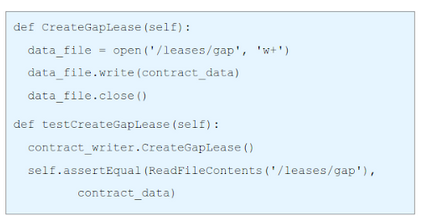
\includegraphics[width=1\textwidth]{esempioFlaky}
	\caption{\emph{Esempio flaky test}}
	\label{fig:fig1.1}
\end{figure}

Il metodo “\emph{CreateGapLease}” apre il file “\emph{/leases/gap}” ed esegue la scrittura del contenuto della variabile “\emph{contract\_data}” al suo interno ed infine chiude il file.
Il test case “\emph{testCreateGapLease}” invoca la funzione “\emph{CreateGapLease}” e successivamente controlla che il contenuto del file “\emph{/leases/gap}” sia effettivamente
uguale al contenuto della variabile “\emph{contract\_data}”.
Ma cosa avviene nel momento in cui il file “\emph{/leases/gap}” esiste già e contiene già dati al suo interno? In questo caso il test genererà un fail. In questo caso il flaky
è dovuto semplicemente ad un errato controllo della precondizione del test, ma in generale errori di questo tipo possono capitare nei casi più disparati (es. in ambito di concorrenza, network etc.).
Una prima strategia di fix può essere quella di verificare l’effettiva esistenza del file “\emph{/leases/gap}” (eliminandolo in caso affermativo).
La figura \ref{fig:fig1.2} mostra il codice del metodo “testCreateGapLease” dopo la modifica.
\begin{figure}[h]
	\centering
	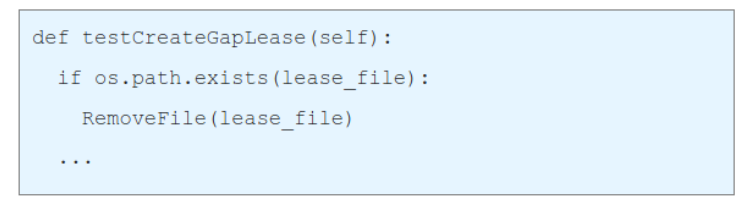
\includegraphics[width=1\textwidth]{figura1.2}
	\caption{\emph{Snippet di codice modificato}}
	\label{fig:fig1.2}
\end{figure}

Tuttavia, neanche questa modifica è sufficiente per garantire la corretta esecuzione del caso di test in quanto, se “\emph{/leases/gap}” ha un path di tipo NFS e può essere scritto da un altro test, il metodo “\emph{testCreateGapLease}” può ancora fallire improvvisamente. La soluzione in questo caso consiste nell’effettuare alcune piccole modifiche al codice del metodo “\emph{CreateGapLease}” per rendere unica la
risorsa di cui ha bisogno.

La figura \ref{fig:fig.1.3} mostra il codice del metodo “\emph{CreateGapLease}” dopo aver effettuato le opportune modifiche.
\newpage
\begin{figure}[h!]
	\centering
	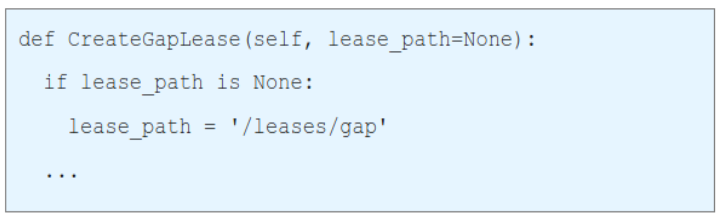
\includegraphics[width=1\textwidth]{figura1.3}
	\caption{\emph{Codice modificato}}
	\label{fig:fig.1.3}
\end{figure}

La chiamata al metodo “CreateGapLease” verrà effettuata nello stesso modo illustrato precedentemente, ma il test potrà passargli un path differente. Tale strategia impedirà fallimenti ad intermittenza del test case.

La figura \ref{fig:fig.1.4} mostra il codice del metodo nella sua versione finale\textsuperscript{[6]}.
\begin{figure}[h!]
	\centering
	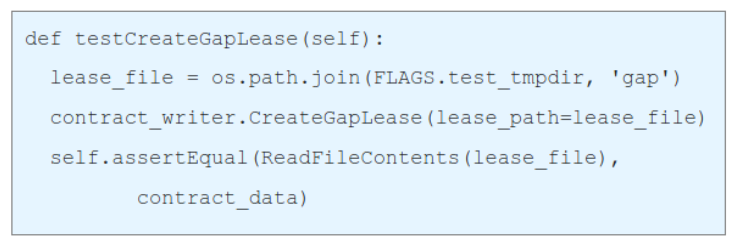
\includegraphics[width=1\textwidth]{figura1.4}
	\caption{\emph{Versione finale del codice}}
	\label{fig:fig.1.4}
\end{figure}
\chapter{CAPITOLO 2}
\fancyhead[L]{CAPITOLO 2}
\fancyhead[C]{}
\section{Mapping}
I mapping study sono effettuati per avere un quadro completo
delle conoscenze attualmente disponibili in una certa area di ricerca. Il mapping viene eseguito attraverso il conteggio dei contributori in relazione alle categorie che sono state approfondite. Un mapping ha lo scopo di approfondire quali argomenti
sono stati trattati e dov’è possibile reperire tali informazioni. Essendo però un processo sistematico, condivide molte delle metodologie di una revisione sistematica della letteratura. Quello che però fa discostare un mapping da una
\emph{systematic review} sono gli obiettivi finali: durante una revisione sistematica si punta a sintetizzare delle evidenze in un determinato campo di analisi, nello studio delle
mappature sistematiche l’obiettivo è piuttosto definire un'area di ricerca.
Per definire un mapping sistematico, \textbf{Petersen et al}.[4] propongono di seguire la seguente linea guida:
\begin{itemize}
	\item Domande di ricerca: Individuare le domande per le quali ricercare una risposta. Tali domande guideranno tutto lo studio;
	\item Ricerca della documentazione: Individuare le parole chiave più opportune da formulare per effettuare la fase di ricerca;
	\item Criteri di inclusione/esclusione: Individuare dei criteri per scartare risultati non inerenti allo studio;
	\item Valutazione della qualità: Valutare i risultati in base alla loro qualità;
	\item Estrazione dei dati: Sintetizzare i risultati in base alle domande di ricerca che sono state poste;
	\item Analisi e classificazione: Visualizzare le informazioni di ogni item di ricerca e raggrupparle in base a caratteristiche comuni;
	\item Validazione: Descrivere eventuali minacce dello studio condotto e valutare la ripetibilità dello studio.
\end{itemize}
\section{Mapping study flaky test}
\subsection{Domande di ricerca}
La prima fase per effettuare il mapping study legato alla problematica dei \emph{flaky test} è stata l’individuazione delle domande di ricerca. Sono state quindi poste
le seguenti domande:
\begin{enumerate}[start=0,label={(\bfseries RQ\arabic*):}]
	\item È stato rilasciato un dataset?
	\item Hanno lavorato anche su progetti closed source?
	\item Viene detto in che linguaggio di programmazione sono scritti i progetti utilizzati?
	\item Viene descritto che tipo di sistema di building utilizzano?
	\item Sono state definite le tecniche che hanno utilizzato per sviluppare il dataset?
	\item Vengono definite quali sono le root cause più frequenti che sono state individuate?
	\item Viene definito che metodo empirico hanno utilizzato per individuare le root cause?
	\item Viene detto a chi è indirizzata questa ricerca?
	\item In che anno è stata pubblicata la ricerca?
\end{enumerate}

Dopo aver individuato le domande di ricerca, si è passati a identificare le stringhe da utilizzare. Per poterle individuare è stato seguito il modello PICO (\emph{Population, Intervention, Comparison and Outcomes}) sviluppato da \textbf{Kitchenham} e \emph{Charters} che ha portato ai seguenti risultati:
\begin{itemize}
	\item \emph{Population}: Ingegneri del software;
	\item \emph{Intervention}: Continuous integration;
	\item \emph{Comparison}: Strategie per identificare i flaky test e comparare la costruzione di dataset per progetti open source e closed source;
	\item \emph{Outcomes}: comprendere lo stato dell’arte e le cose che sono state fatte.
\end{itemize}

Tramite questo modello, sono state individuate le seguenti keywords: \emph{“Software testing”, “Continuous Integration”, “Flaky test”, “dataset”, “open source”, “closed source”}.

Successivamente sono stati individuati tre tra i più importanti databases per la raccolta di dati in letteratura, ovvero \textbf{IEEE}, \textbf{ACM} e \textbf{Scopus} e sono state formulate le seguenti query.
\newpage
\begin{table}[h!]
	\centering
	\scalebox{0.7}{\begin{tabular}{|l|l|}
		\hline
		\textbf{Database} & \textbf{Search}                                                                                                                                                                                                                                                                                                                                                                                                                                                                                                         \\ \hline
		IEEE              & \begin{tabular}[c]{@{}l@{}}((("flaky" OR "flakiness" OR "test pass and fail" \\ OR "non deterministic") AND "test" AND \\ ("SE" OR "software engineering" OR\\  "computer science")) AND \\ ((("dataset" OR "database")OR\\  ("project open source" OR \\ "close* source" OR "source code"))OR\\  ("build* system*" OR \\ "maven" OR "gradle" OR\\  "continuous integration" OR\\  "integration")OR ("root cause" AND \\ ("detect*" OR "improve*"))))\end{tabular}                                                      \\ \hline
		ACM               & \begin{tabular}[c]{@{}l@{}}((("flaky" OR "flakiness" OR\\  "test pass and fail" OR\\  "non deterministic test*") AND\\  "test" AND\\  ("SE" OR "software engineering" OR\\  "computer science")) AND\\  ((("dataset" OR "database" OR\\  "db")OR ("project open source" OR\\  "close* source" OR "source code")) OR\\  ("build* system*" OR "maven" OR\\  "gradle" OR "building" OR\\  "continuous integration" OR\\  "travis" OR "integration test") OR\\  ("root cause" AND ("detect*" OR "improve*"))))\end{tabular} \\ \hline
		Scopus            & \begin{tabular}[c]{@{}l@{}}((("flaky" OR "flakiness" OR \\ "test pass and fail" OR\\  "non deterministic test*") AND\\  "test" AND ("SE" OR\\  "software engineering" OR\\  "computer science"))AND\\  ((("dataset" OR "database" OR\\  "db")OR ("project open source" OR\\  "close* source" OR "source code"))OR\\  ("build* system*" OR "maven" OR\\  "gradle" OR "building" OR\\  "continuous integration" OR\\  "travis" OR "integration test")OR\\  ("root cause" AND ("detect*" OR "improve*"))))\end{tabular}    \\ \hline
	\end{tabular}}
\end{table}

E sono stati ottenuti seguenti risultati:
\newpage
\begin{table}[h!]
	\centering
	\begin{tabular}{|c|c|}
		\hline
		\multicolumn{1}{|l|}{\textbf{Database}} & \multicolumn{1}{l|}{\textbf{\#Results}} \\ \hline
		IEEE                                    & 13                                      \\ \hline
		ACM                                     & 153                                     \\ \hline
		Scopus                                  & 137                                     \\ \hline
		Total                                   & 303                                     \\ \hline
	\end{tabular}
\end{table}
\subsection{Criteri di inclusione/esclusione}
Per ogni artefatto sono state riportate su un foglio di calcolo le seguenti informazioni:
	\begin{table}[h]
		\scalebox{0.7}{\begin{tabular}{|l|l|l|l|l|l|l|}
			\hline
			Paper name & Item type & Database & Authors & Publication year & Publication title & Notes \\ \hline
		\end{tabular}}
	\end{table}

Sono state successivamente eseguite le seguenti fasi:
\begin{itemize}
	\item Eliminare gli articoli ripetuti (45 articoli);
	\item Eliminare gli articoli precedenti agli anni 2000 (6 articoli).
\end{itemize}

Con tale tecnica è stato possibile ridurre gli articoli da analizzare da 303 ad un totale di 252. Successivamente sono stati letti sia il titolo che l’abstract di ogni artefatto e si è deciso di scartare tutti gli articoli che non presentavano dei riferimenti diretti all’argomento trattato. Tale fase ha permesso di eliminare dalla lista 202 artefatti, ottenendo così un totale di 50 articoli.

Si è passata poi alla lettura totale degli articoli rimanenti. Grazie a questa fase sono stati eliminati venti artefatti poiché non erano pertinenti allo studio o lo erano solo in minima parte. Successivamente sono stati riletti tutti gli articoli scartati dalle fasi precedenti e si è ritenuto di riprendere in considerazione uno degli artefatti scartati. Tale tecnica ha permesso di avere nella lista trentuno articoli in totale.
\subsection{Snowball}
Dopo aver fatto una prima seleziona degli artefatti di interesse per il mapping sistematica, è stata applicata la tecnica dello “\emph{snowballing}”; tale tecnica consiste nel leggere le “\emph{reference}” di ogni articolo finora considerato, con lo scopo di individuare qualche artefatto che possa essere ritenuto d’interesse per la ricerca, ma che non è ancora stato preso in considerazione. La tecnica è stata applicata sui trentuno articoli e sono stati così individuati altri tre artefatti. Oltre ai tre articoli, sono stati tenuti in considerazione anche nove siti web citati nelle \emph{reference} che hanno permesso di avere un quadro completo della problematica. La tecnica dello snowballing ha permesso quindi di incrementare la lista totale degli articoli portandola ad un totale di trentaquattro.
\subsection{Valutazione della qualità}
Nel processo di valutazione della qualità, sono stati identificati dei criteri per valutare la qualità degli articoli presi in considerazione. Lo scopo di questa fase è quella di eliminare dalla lista tutti gli articoli che non soddisfano i criteri minimi di qualità richiesti.

Sono state così definite le seguenti domande:
\begin{enumerate}[start=0,label={(\bfseries R\arabic*):}]
	\item Gli obiettivi sono chiaramente indicati?
	\item Quanto sono credibili i risultati?
	\item I partecipanti allo studio o le unità di osservazione sono state adeguatamente descritte?
	\item Se lo studio prevede la valutazione di una tecnologia, essa è stata chiaramente identificata?
	\item Tutte le domande dello studio hanno una risposta?
	\item Sono presentati tutti i risultati?
	\item I metodi di raccolta dei dati sono descritti in modo adeguato?
\end{enumerate}

Per ognuna delle seguenti domande è stato assegnato un intervallo compreso tra 0 ed 1 per l’eventuale risposta. La seguente tabella mostra gli intervalli individuati per la valutazione di ogni domanda.

\begin{table}[h]
	\centering
	\begin{tabular}{|c|c|}
		\hline
		\textbf{Legenda} & \textbf{}    \\ \hline
		0.0              & No           \\ \hline
		0.1 - 0.3        & Raramente    \\ \hline
		0.4 - 0.6        & Parzialmente \\ \hline
		0.7 - 0.9        & Abbastanza   \\ \hline
		1.0              & Si           \\ \hline
	\end{tabular}
\end{table}

Il punteggio totale è stato ottenuto tramite la somma del punteggio assegnato a ogni domanda. Si è deciso di prendere in considerazione solo gli articoli che hanno raggiunto uno standard di qualità almeno pari a “parziale”.

La seguente tabella mostra gli intervalli che sono stati individuati per valutare la qualità totale di ogni artefatto.

\begin{table}[h]
	\centering
	\begin{tabular}{|c|c|}
		\hline
		\textbf{Legenda}  & \textbf{}    \\ \hline
		0.0               & No           \\ \hline
		0.1 - 2.1         & Raramente    \\ \hline
		\rowcolor[HTML]{34FF34} 
		2.2 - 4.5         & Parzialmente \\ \hline
		\rowcolor[HTML]{34FF34} 
		4.6 - 6.2         & Abbastanza   \\ \hline
		\rowcolor[HTML]{34FF34} 
		\textgreater{}6.3 & Si           \\ \hline
	\end{tabular}
\end{table}

Di seguito sono mostrati i risultati che si sono ottenuti da tutti gli artefatti analizzati, mentre nell’Appendice A sono riportati i riferimenti degli articoli studiati con il relativo codice.
\newpage
\begin{table}[h]
	\centering
		\scalebox{0.65}{

			\begin{tabular}{|l|l|}
		\hline
		\textbf{Study No.} & \textbf{}  \\ \hline
		S1                 & Si         \\ \hline
		S2                 & Abbastanza \\ \hline
		S3                 & Abbastanza \\ \hline
		S4                 & Abbastanza \\ \hline
		S5                 & Abbastanza \\ \hline
		S6                 & Abbastanza \\ \hline
		\rowcolor[HTML]{FD6864} 
		S7                 & Raramente  \\ \hline
		\rowcolor[HTML]{FD6864} 
		S8                 & Raramente  \\ \hline
		S9                 & Abbastanza \\ \hline
		S10                & Abbastanza \\ \hline
		S11                & Si         \\ \hline
		S12                & Abbastanza \\ \hline
		S13                & Si         \\ \hline
		S14                & Si         \\ \hline
		S15                & Si         \\ \hline
		S16                & Si         \\ \hline
		S17                & Abbastanza \\ \hline
		S18                & Si         \\ \hline
		S19                & Si         \\ \hline
		S20                & Abbastanza \\ \hline
		S21                & Si         \\ \hline
		S22                & Si         \\ \hline
		S23                & Abbastanza \\ \hline
		S24                & Si         \\ \hline
		S25                & Si         \\ \hline
		\rowcolor[HTML]{FD6864} 
		S26                & Raramente  \\ \hline
		
		S27                & Si         \\ \hline
		S28                & Abbastanza \\ \hline
		S29                & Abbastanza \\ \hline
		S30                & Abbastanza \\ \hline
		S31                & Si         \\ \hline
		S32                & Abbastanza \\ \hline
		S33                & Abbastanza \\ \hline
		\rowcolor[HTML]{FD6864} 
		S34                & Raramente  \\ \hline
		\rowcolor[HTML]{FD6864} 
	\end{tabular} }
\end{table}

Dalla valutazione della qualità è emerso che quattro articoli non soddisfano la soglia minima di accettazione. Si è quindi deciso di eliminare dall’elenco gli artefatti numero S7, S8, S26 e S34 e di continuare le successive fasi sui restanti trenta artefatti e i nove siti web.
\subsection{Estrazione dei dati}
Per la fase di estrazione dei dati è stata effettuata seguendo il modello proposto da \textbf{Petersen et al}.

In questa fase è stata generata una tabella contenente tutti gli studi che sono stati presi in considerazione con le rispettive domande di ricerca a cui rispondevano.

La tabella sottostante sintetizza i risultati che sono stati ottenuti analizzando ogni articolo.
% Please add the following required packages to your document preamble:
% \usepackage[table,xcdraw]{xcolor}
% If you use beamer only pass "xcolor=table" option, i.e. \documentclass[xcolor=table]{beamer}
\begin{table}[h]
	\begin{tabular}{|
			>{\columncolor[HTML]{EFEFEF}}l |
			>{\columncolor[HTML]{EFEFEF}}l |
			>{\columncolor[HTML]{EFEFEF}}l |
			>{\columncolor[HTML]{EFEFEF}}l |
			>{\columncolor[HTML]{EFEFEF}}l |
			>{\columncolor[HTML]{EFEFEF}}l |
			>{\columncolor[HTML]{EFEFEF}}l |
			>{\columncolor[HTML]{EFEFEF}}l |
			>{\columncolor[HTML]{EFEFEF}}l |
			>{\columncolor[HTML]{EFEFEF}}l |}
		\hline
		\textbf{Study} & \textbf{Anno} & \textbf{RQ1} & \textbf{RQ2} & \textbf{RQ3} & \textbf{RQ4} & \textbf{RQ5} & \textbf{RQ6} & \textbf{RQ7} & \textbf{RQ8} \\ \hline
		S1             & 2014          & -            & X            & -            & X            & X            & X            & -            & -            \\ \hline
		S2             & 2015          & -            & X            & X            & X            & X            & X            & -            & X            \\ \hline
		S3             & 2015          & -            & X            & -            & -            & -            & -            & -            & -            \\ \hline
		S4             & 2015          & -            & X            & -            & -            & -            & -            & -            & -            \\ \hline
		S5             & 2015          & -            & X            & X            & X            & -            & -            & -            & -            \\ \hline
		S6             & 2015          & -            & X            & -            & -            & -            & -            & -            & -            \\ \hline
		S7             & 2016          & -            & X            & -            & -            & -            & -            & -            & X            \\ \hline
		S8             & 2017          & -            & X            & -            & X            & -            & -            & -            & -            \\ \hline
		S9             & 2017          & -            & X            & X            & X            & -            & -            & -            & -            \\ \hline
		S10            & 2017          & -            & -            & -            & -            & X            & X            & -            & -            \\ \hline
		S11            & 2017          & -            & X            & -            & X            & -            & -            & -            & -            \\ \hline
		S12            & 2018          & X            & X            & X            & X            & -            & X            & -            & X            \\ \hline
		S13            & 2018          & -            & X            & X            & X            & X            & X            & X            & -            \\ \hline
		S14            & 2018          & -            & X            & -            & X            & -            & -            & -            & -            \\ \hline
		S15            & 2018          & -            & -            & -            & -            & -            & X            & -            & -            \\ \hline
		S16            & 2019          & -            & -            & -            & -            & X            & X            & -            & X            \\ \hline
		S17            & 2019          & -            & X            & -            & X            & X            & X            & -            & X            \\ \hline
		S18            & 2019          & -            & -            & -            & -            & -            & -            & -            & -            \\ \hline
		S19            & 2019          & -            & X            & -            & -            & -            & -            & -            & -            \\ \hline
	\end{tabular}
\end{table}
\newpage
\begin{table}[h]
	\begin{tabular}{{|
				>{\columncolor[HTML]{EFEFEF}}l |
				>{\columncolor[HTML]{EFEFEF}}l |
				>{\columncolor[HTML]{EFEFEF}}l |
				>{\columncolor[HTML]{EFEFEF}}l |
				>{\columncolor[HTML]{EFEFEF}}l |
				>{\columncolor[HTML]{EFEFEF}}l |
				>{\columncolor[HTML]{EFEFEF}}l |
				>{\columncolor[HTML]{EFEFEF}}l |
				>{\columncolor[HTML]{EFEFEF}}l |
				>{\columncolor[HTML]{EFEFEF}}l |}}
	\hline
	\textbf{Study} & \textbf{Anno} & \textbf{RQ1} & \textbf{RQ2} & \textbf{RQ3} & \textbf{RQ4} & \textbf{RQ5} & \textbf{RQ6} & \textbf{RQ7} & \textbf{RQ8} \\ \hline
		S20 & 2019 & X & X & X & X & \- & X & - & - \\ \hline
		S21 & 2019 & - & X & - & - & -          & - & -          & - \\ \hline
		S22 & 2019 & X & X & X & X & -          & X & -          & - \\ \hline
		S23 & 2019 & - & X & - & - & -          & - & -          & - \\ \hline
		S24 & 2019 & - & X & X & - & -          & - & -          & - \\ \hline
		S25 & 2019 & - & - & - & - & -          & - & -          & - \\ \hline
		S26 & 2019 & - & X & - & - & X          & X & -          & - \\ \hline
		S27 & 2019 & - & X & - & - & -          & - & -          & - \\ \hline
		S28 & 2019 & X & X & X & X & X          & X & -          & - \\ \hline
		S29 & 2019 & - & X & - & - & X          & X & -          & - \\ \hline
		S30 & 2019 & - & - & - & - & X          & X & -          & - \\ \hline
	\end{tabular}
\end{table}

Il grafico in figura \ref{fig:fig.2.1} sintetizza tutte le fasi che sono state effettuate per la selezione degli artefatti utili per il mapping sistematico.
\newpage
\begin{figure}[h]
	\centering
	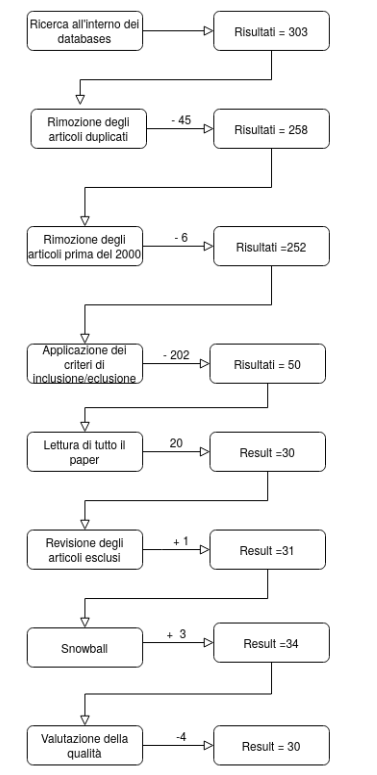
\includegraphics[height=0.6\textheight]{figura1.5}
	\caption{\emph{Sintesi della selezione degli articoli}}
	\label{fig:fig.2.1}
\end{figure}
\newpage
\subsection{Minacce alla validità}
\subsubsection{Minaccia alla validità descrittiva}
La validità descrittiva è la misura con cui le osservazioni sono descritte in maniera accurata ed oggettiva. Questo tipo di minaccia è solitamente maggiore negli studi di tipo qualitativo rispetto a quelli di tipo quantitativo. Questa minaccia quindi viene considerata sotto controllo.
\subsubsection{Minaccia alla validità teorica}
La validità teorica è data dalla capacità dell’autore che ha effettuato il mapping study di “cogliere” quello che gli autori degli articoli volevano effettivamente dimostrare. Il fattore che gioca un ruolo fondamentale all’interno di questa minaccia è il pregiudizio che si può avere su determinati autori che a loro
volta influenzano gli articoli da analizzare.

Un'altra minaccia alla validità teorica può derivare dalla formulazione delle
query che potrebbero aver portato a non includere alcuni risultati importanti ai fini dello studio.

Per mitigare questa minaccia si è deciso di applicare la tecnica dello
\emph{snowballing} su tutti gli articoli che sono stati selezionati durante la fase di analisi.
La tecnica ha infatti il fine di individuare artefatti utili che possono essere stati non considerati durante la fase di ricerca.

Infine, la fase di estrazione dei dati effettuata da un singolo ricercatore potrebbe aver portato a non considerare studi importanti. Per mitigare questa minaccia è stato chiesto ad esperto del dominio applicativo ma esterno alla ricerca
di valutare eventuali studi ritenuti dal primo autore “poco chiari”.
\subsubsection{Generalizzazione}
\textbf{Petersen et al}. effettuano una distinzione tra la generalizzazione esterna ed interna. Con la prima si intende la generalizzazione tra gruppi o organizzazioni, mentre con la seconda si indica la generalizzazione all’interno di un singolo gruppo.
I risultati ottenuti potrebbero non essere applicabili all’interno di una revisione sistematica della letteratura poiché gli obiettivi delle ricerche sono differenti.

Tuttavia, visto che si è seguito un approccio di tipo sistematico, gran parte delle
strategie di ricerca risulta in comune, pertanto questa minaccia si ritiene mitigata.
\subsubsection{Validità di interpretazione}
La validità di interpretazione viene raggiunta quando le conclusioni che sono state tratte dai dati risultano essere ragionevoli. Una delle minacce di interpretazione dei dati può essere dovuta al pregiudizio che l’autore del mapping ha verso alcune conclusioni che sono state mostrate nei differenti artefatti. Per mitigare tale minaccia è stato chiesto ad un esperto del dominio applicativo ma esterno alla ricerca di dare un parere sulla veridicità dei dati presi in esame.
\subsubsection{Ripetibilità}
È stato effettuato un mapping study sistematico proprio al fine di garantire la ripetibilità di tutto ciò che si è fatto. Sono state inoltre seguite le linee guida dettate
da \textbf{Kai Petersen, Sairam Vakkalanka et al}. all’interno dell’articolo “\emph{Guidelines
for conducting systematic mapping studies in software engineering: An update}”.

Sono inoltre dettagliate tutte le fasi seguite con assoluto rigore, pertanto tale minaccia risulta mitigata.
\subsection{Analisi dei dati e classificazione}
L’obiettivo dell’analisi dei dati e della classificazione è anche quello di organizzare a livello visivo le informazioni estratte dalle varie domande di ricerca,
in modo che esse possano essere rapidamente individuate e comprese. Le informazioni su ogni articolo sono state mappate ed illustrate visivamente attraverso l’utilizzo di grafici e diagrammi. Successivamente è stato assegnato una categoria ad ogni artefatto e si è passati quindi alla fase di conteggio.
\subsubsection{Numero di dataset (RQ1)}
Dalla prima domanda di ricerca è emerso che in quasi tutti gli studi non è
stato rilasciato un dataset.

Gli unici dataset che sono stati rilasciati (in totale quattro) rientrano nel periodo 2018-2019; questo dato è indice di un argomento di ricerca poco conosciuto e che necessita di ulteriori sviluppi.

Il grafico in figura \ref{fig:fig.2.2} mostra la frequenza di pubblicazione dei dataset messi a disposizione.
\begin{figure}[h]
	\centering
	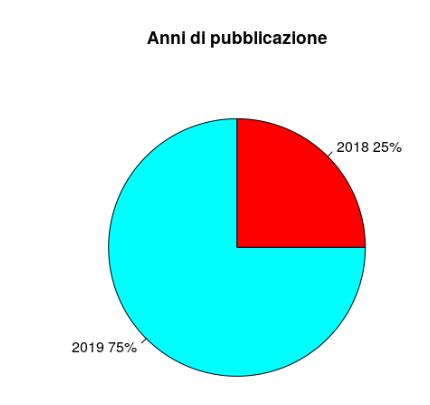
\includegraphics[width=0.7\textwidth]{1.6}
	\caption{\emph{Frequenza di pubblicazione del dataset}}
	\label{fig:fig.2.2}
\end{figure}

Dal grafico è emerso che quasi la totalità dei dataset messi a disposizione
sono stati implementati nel corso del 2019 (75\%). Il numero dei dataset risulta essere comunque molto esiguo.

\subsubsection{Lavoro su progetti closed source (RQ2)}
Dalla seconda domanda di ricerca è emerso che la quasi totalità degli studi effettuati non ha considerato progetti closed-source nella loro valutazione e in alcuni articoli questa problematica è stata considerata solo come minaccia per la validità.

Il grafico in figura \ref{fig:fig2.3} mostra il numero di studi sui quali sono state effettuate ricerche anche su progetti closed-source suddivisi per anno.
\newpage
\begin{figure}[h!]
	\centering
	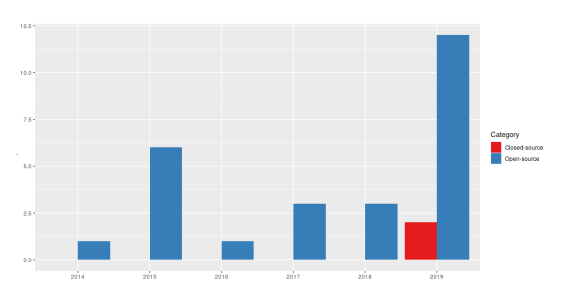
\includegraphics[width=1\textwidth]{2.3}
	\caption{\emph{Numero di progetti su cui sono stati condotti gli studi}}
	\label{fig:fig2.3}
\end{figure}
\subsubsection{Linguaggi di programmazione utilizzati (RQ3)}
Dall'analisi effettuata risulta che quasi tutti gli articoli analizzati riportano le caratteristiche del linguaggio di programmazione impiegato per definire gli oggetti
sperimentali (ventiquattro su trenta). Di questi, quasi la totalità dei progetti
analizzati è scritta in Java (viene infatti definita come una minaccia in alcuni degli
articoli analizzati, in quanto il linguaggio potrebbe presentare alcune caratteristiche
non comuni a tutti i linguaggi di programmazione). È stata quindi approfondita la problematica per capire quale fosse la distribuzione dei linguaggi di programmazione.

Il grafico in figura \ref{fig:fig.2.4} mostra la frequenza di ogni linguaggio di programmazione.
\newpage
\begin{figure}[h]
	\centering
	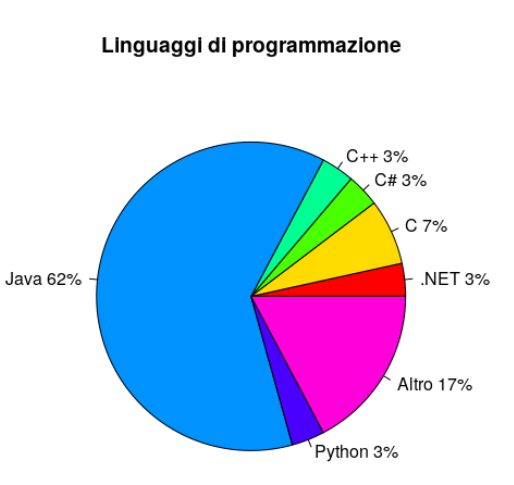
\includegraphics[width=0.7\textwidth]{2.4}
	\caption{\emph{Distribuzione dei linguaggi di programmazione analizzati}}
	\label{fig:fig.2.4}
\end{figure}

È possibile notare che più della metà dei progetti analizzati sono stati sviluppati in Java. Tale dato non stupisce in quanto attualmente il linguaggio Java risulta essere uno dei più utilizzati al mondo. È altresì importante sottolineare che per alcuni linguaggi la problematica è stata trattata solo in minima parte o non è stata per nulla trattata.
\subsubsection{Tipi di build utilizzati (RQ4)}
Dall’analisi effettuata è emerso che non sempre è stato dichiarato
esplicitamente il sistema di build adoperato durante la costruzione del dataset.

Negli articoli in cui tale informazione è presente, il linguaggio di programmazione utilizzato è sempre stato Java. Dei trenta articoli, in nove è stato riportato anche il tipo di build system utilizzato (in alcuni casi anche più di uno).

Il grafico in figura \ref{fig:fig.2.5} mostra la frequenza dei sistemi di building utilizzati
all’interno dei progetti che sono stati testati.
\begin{figure}[h]
	\centering
	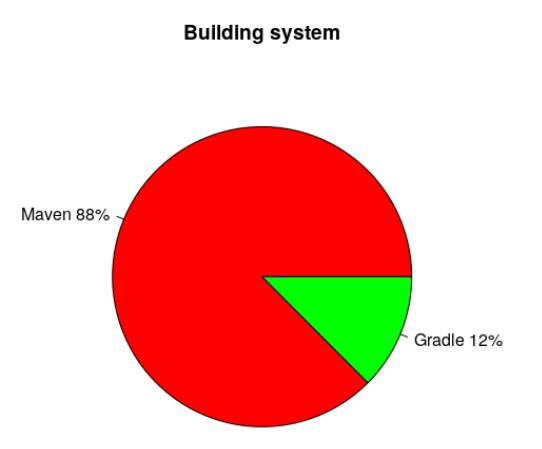
\includegraphics[width=0.7\textwidth]{2.5}
	\caption{\emph{Sistemi di building utilizzati}}
	\label{fig:fig.2.5}
\end{figure}

È possibile notare che quasi la totalità dei progetti analizzati utilizzano come sistema di build Maven (preso in considerazione in sette articoli), mentre solo il 12\% utilizzano Gradle (preso in considerazione in un solo articolo).
\subsubsection{Individuazione del dataset (RQ5)}
In tutti gli articoli in cui è stata dichiarata la costruzione del dataset (diciotto articoli), è stato anche descritto il metodo utilizzato per la descrizione.

La strategia più comune risulta quella di scaricare da GitHub i repository più popolari per poi verificare la presenza di metodi flaky (38\%).

Le altre strategie utilizzate si basano principalmente sull’uso di Travis (valutando lo stato della build oppure i file di log generati) e sul cercare la stringa “flaky” all’interno dei bug report o nei messaggi di commit all’interno del motore di ricerca di GitHub.

Il grafico in figura \ref{fig:fig.2.6} mostra la percentuale di utilizzo di ogni strategia per individuare i dataset.

\begin{figure}[h]
	\centering
	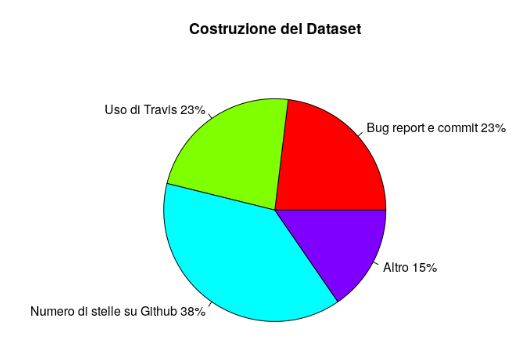
\includegraphics[width=1\textwidth]{2.6}
	\caption{\emph{Strategie usate per la costruzione del dataset}}
	\label{fig:fig.2.6}
\end{figure}
\subsubsection{Quali sono le root cause più frequenti (RQ6)}
Sui trenta articoli esaminati solo in dieci casi sono state individuate le \emph{root cause} dei \emph{flaky test}.

In gran parte degli articoli le root cause risultano le stesse,
ossia: dipendenza dall’ordine, concorrenza, async wait, tempo, rete, random, perdita di risorse, operazioni con numeri float e problemi di I/O.

È però interessante soffermarsi sulle root cause “Output restrittivi” e “Interfaccia grafica”, tali root
cause infatti sono presenti con una percentuale molto bassa (2\%) poiché non sono state mai individuate precedentemente, ma sono frutto di studi effettuati nel 2019. 

Possiamo quindi definirle nel seguente modo:
\begin{itemize}
	\item \emph{Output restrittivi}: Sono degli output validi, ma considerati fuori dai “range” consentiti per questioni di design;
	\item \emph{Interfaccia grafica}: Un’interfaccia grafica viene definita come “flaky” nel momento in cui avviene una mancata comunicazione tra il processo che esegue il rendering e l’interfaccia stessa.
\end{itemize}

La figura \ref{fig:fig.2.7} mostra le root cause più comuni.
\newpage
\begin{figure}[h]
	\centering
	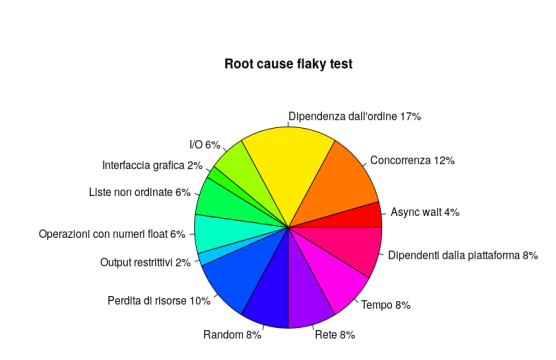
\includegraphics[width=1\textwidth]{2.7}
	\caption{\emph{Root cause dei flaky test}}
	\label{fig:fig.2.7}
\end{figure}
\subsubsection{Metodo empirico per la valutazione delle root cause (RQ7)}
Dagli articoli che rispondono a questa domanda di ricerca sono state estratte le tecniche adoperate per valutare le root cause dei flaky test.

Nel 29\% dei casi, il metodo comunemente utilizzato al momento consiste
nell’effettuare nuovamente l’esecuzione di un caso di test e verificare se quest’ultimo cambia stato rispetto all’esecuzione precedente (pass/fail o viceversa). Le altre strategie adoperate sono:
%AGGIUNGERE BENE I SUBITEM
\begin{itemize}
	\item Strumentazione del codice: Creazione di un codice che monitora comportamenti specifici di una applicazione;
	\item Coverage: Con questa tecnica viene calcolata la coverage (solitamente la line) ogni volta che il caso di test viene eseguito, se si riscontra un cambio di coverage in parti del codice che non sono state modificate, il test viene classificato come flaky;
	\item Analisi del codice: L’analisi del codice può essere eseguita in due modi:
	\subitem Statica: In questo caso gli sviluppatori definiscono un metodo flaky se rilevano che nel codice sorgente del test viene fatto uso di qualche funzione che può generare un flaky;
	\subitem Dinamica: Viene eseguito il codice sorgente del test e si valutano glioutput generati e i file di log scritti. Se si nota una discordanza tra le due esecuzioni, il metodo viene definito flaky.
\end{itemize}

Il grafico in figura \ref{fig:fig.2.8} mostra le frequenze di utilizzo di ogni tecnica che è stata descritta precedentemente.
\newpage
\begin{figure}[h]
	\centering
	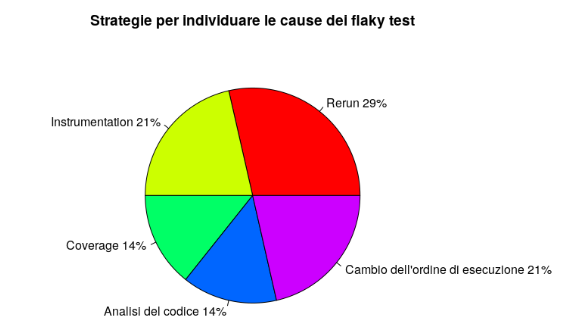
\includegraphics[width=1\textwidth]{2.8}
	\caption{\emph{Strategia per individuare i flaky test}}
	\label{fig:fig.2.8}
\end{figure}
\subsubsection{A chi viene indirizzata la ricerca mostrata nei diversi studi (RQ8)}
Dall'analisi effettuata è emerso che in cinque artefatti è chiaramente indicato a chi fosse rivolto lo studio (grandi aziende e ambito accademico); invece, nei restanti artefatti si può intuire che lo studio è rivolto ad un pubblico prettamente accademico.

La figura \ref{fig:fig.2.9} mostra la percentuale degli articoli dove vengono menzionati sia le aziende che gli accademici come fruitori finali dello studio, comparato a quelli dove vengono citati solo gli accademici.\newpage
\begin{figure}[h]
	\centering
	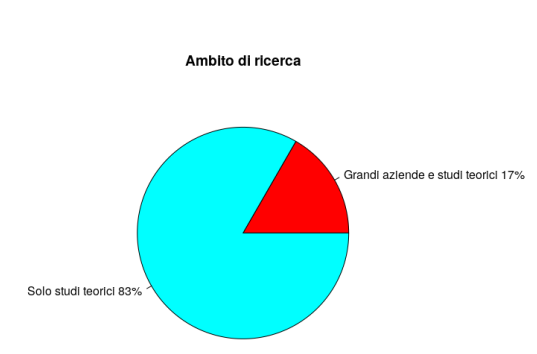
\includegraphics[width=1\textwidth]{2.9}
	\caption{\emph{Ambito di ricerca per ogni artefatto}}
	\label{fig:fig.2.9}
\end{figure}

È interessante soffermarsi su quest’ultima percentuale poiché nonostante il problema sia stato posto inizialmente dalle grandi aziende (Google, Facebook, Huawei in primis), esso è diventato un argomento su cui sono nati molteplici studi da parte degli accademici.
\subsubsection{Anno di pubblicazione (RQ9)}
Gran parte degli studi sono stati pubblicati tra il 2018 e il 2019 (il 63\%), questo ci suggerisce che l’argomento rappresenta una problematica attuale ed è tuttora molto studiato.
La figura \ref{fig:fig.2.10} mostra la frequenza di pubblicazione degli artefatti suddivisa per anni.
\newpage
\begin{figure}[h]
	\centering
	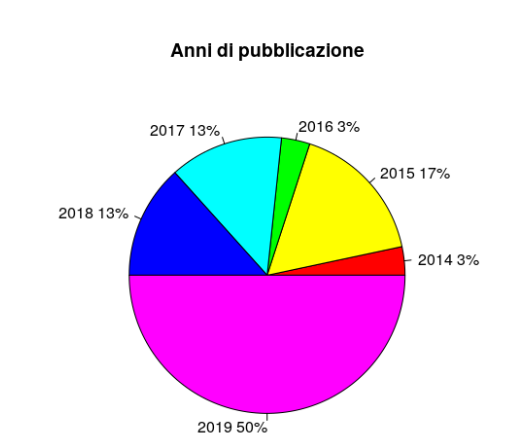
\includegraphics[width=1\textwidth]{2.10}
	\caption{\emph{Frequenza di pubblicazione suddivisa per anni}}
	\label{fig:fig.2.10}
\end{figure}
\subsection{Conclusioni}
	Dallo studio effettuato è emerso che:
\begin{itemize}

	\item  Gli unici studi sui quali sono stati effettivamente rilasciati dei dataset sono
	solo quelli presentati tra il 2018 e il 2019, tale dato ci porta a sottolineare l’importanza e la necessità da parte sia delle aziende che degli accademici
	di rilasciare nuovi dati o di ampliare quelli già esistenti;
	\item Bisogna analizzare con particolare attenzione anche progetti closed-source
	poiché le dinamiche e i meccanismi con cui vengono costruiti tali progetti possono essere completamente differenti da quelle open-source;
	\item Occorre prestare maggiore attenzione anche ad altri tipi di linguaggi di programmazione, poiché gran parte degli studi sono stati effettuati soltanto
	su progetti scritti in Java e che utilizzano Maven come build system;
	\item  L’uso di GitHub per individuare progetti open-source affetti da flakiness è effettivamente un buon punto di partenza ma bisognerebbe analizzare anche
	repository private o progetti closed-source;
	\item  Negli anni le root cause individuate sono state ampliate per comprendere nuove piattaforme mai considerate in precedenza (es. Android); tale
	ampliamento ha permesso di considerare all’interno delle root cause anche problemi legati all’hardware (es. fotocamera non disponibile). Attualmente questi problemi sono ancora classificati all’interno della causa “problemi
	dipendenti dalla piattaforma”, ma non si esclude che possano diventare una nuova categoria in futuro.
\end{itemize}

\chapter{Capitolo 3}
\fancyhead[L]{CAPITOLO 3}
\fancyhead[C]{}
\section{Creazione del dataset}
Dall’analisi effettuata nel capitolo precedente sono emerse diverse criticità nello studio dei \emph{flaky test}. Tali criticità sono sinonimo di un argomento di ricerca ancora molto da approfondire. Le problematiche maggiori che sono state sono evidenziate all’interno della ricerca sono principalmente legate alla carenza di dati
messi a disposizione per la comunità. Infatti, in molti degli studi precedentemente analizzati, la carenza di dati viene considerata una minaccia alla validità poiché i progetti considerati sono quasi tutti scritti in linguaggio \textbf{Java} ed usano \textbf{Maven} come
sistema di building. Avere diverse tipologie di dataset risulta estremamente importante in quanto tale problematica risulta ancora di notevole interesse da parte delle grandi multinazionali che ogni giorno sviluppano centinaia di progetti utilizzando differenti linguaggi di programmazione.

Nel 2019, nell’ambito della conferenza “\emph{Testing and Verification Symposium}” organizzata da Facebook, sono stati proposte diverse idee innovative che potessero in qualche modo far fronte alla problematica flakiness. Tra le idee
maggiormente apprezzate è possibile citare: “\emph{A scalable infrastructure for fuzzy-driven root causing of flaky tests}” ideato da Filomena Ferrucci (Università di Salerno), Pasquale Salza (Università di Zurigo) e Valerio Terragni (Università della
Svizzera italiana).

La loro idea prevede un nuovo approccio per identificare le \emph{root cause} di un \emph{flaky test}, che non prevede nessun tipo di “\emph{instrumentation}” del codice, ma va ad
identificare la \emph{root cause} dei flaky test, eseguendo il caso di test in differenti configurazioni definite da cluster. Ogni cluster esplora attivamente uno specifico
spazio di esecuzione \textbf{non deterministico}. Il cluster che mostrerà i risultati più
bilanciati tra “pass” e “fail” sarà utilizzato per identificare la root cause di quello
specifico \emph{flaky test}. Il primo passo da fare per sviluppare questo nuovo tool è creare un nuovo dataset con quanti più \textbf{flaky} test possibili.
\section{Approccio alla problematica}
L’idea di base è stata quella di partire da un dataset già esistente, ossia quello
rilasciato dagli sviluppatori di \textbf{iDFlakies}, ed ampliarlo con nuove informazioni.
Questo framework, rilasciato nel 2019 permette l’individuazione di un \emph{flaky test} con una classificazione parziale (dipendente dall’ordine e indipendente dall’ordine).

Il dataset rilasciato con questo framework conta al suo interno
quattrocentoventidue \emph{flaky test}, di cui il 50.5\% sono dipendenti dall’ordine, mentre i restanti 49.5\% sono non dipendenti dall’ordine.
L’individuazione dei \emph{flaky test} all’interno del tool di \textbf{iDFlakies} avviene tramite una serie di configurazioni che cambiano l’ordine di esecuzione sia delle classi di test che dei test case al loro interno.
Tra le configurazioni presenti all’interno di \textbf{iDFlakies}, possiamo citare:
\begin{itemize}
	\item \emph{Original-order}: Esegue tutti i casi di test nell’ordine in cui sono stati scritti
	dallo sviluppatore;
	\item \emph{Random-Class}: Esegue le classi della suite di test in ordine pseudo-casuale, ma mantenendo l’ordine originale di esecuzione dei test all’interno di ogni classe;
	\item \emph{Random-class-method}: Esegue gerarchicamente prima in ordine pseudo-casuale le classi che compongono la test suite per poi eseguire in maniera pseudo-casuale i singoli casi di test che compongono le varie classi;
	\item \emph{Reverse-class}: Inverte l’ordine di esecuzione delle classi di test ma mantiene invariato l’ordine di esecuzione dei singoli test all’interno della classe;
	\item \emph{Reverse-class-method}: Inverte l’ordine sia delle classi di test che dei metodi di test al suo interno.
\end{itemize}

Analizzando il dataset messo a disposizione è emerso che ogni progetto contiene le informazioni presentate nella tabella sottostante:
\begin{table}[h]
	\centering
	\scalebox{0.8}{
	\begin{tabular}{|l|l|l|l|l|l|l|}
		\hline
		\textbf{URL} & \textbf{SHA} & \textbf{Test count} & \textbf{Module Name} & \textbf{Test Name} & \textbf{Category} & \textbf{Version} \\ \hline
	\end{tabular}}
\end{table}
La figura \ref{fig:datasetRilasciato} mostra un esempio per descrivere il contenuto del dataset
rilasciato.
\newpage
\begin{figure}[h]
	\centering
	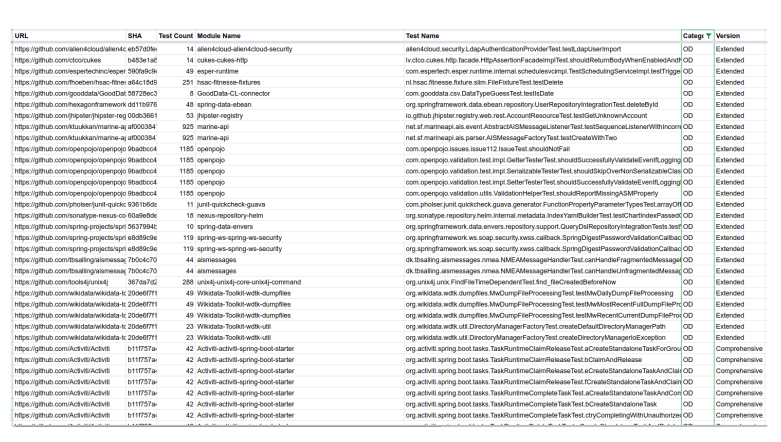
\includegraphics[width=1\textwidth]{3.1}
	\caption{\emph{Parte del dataset di IDFlakies}}
	\label{fig:datasetRilasciato}
\end{figure}
Questo framework recupera il link e lo sha di ogni repository e crea
un’immagine Docker\footnote{Docker è un progetto open-source che automatizza il deployment di applicazioni all'interno di contenitori software, fornendo un'astrazione aggiuntiva grazie alla virtualizzazione a livello di sistema operativo di Linux.}. Una volta scaricato il progetto, prova ad eseguire una delle configurazioni sopra descritte su una delle immagini Docker appena create. È possibile inoltre settare \emph{iDFlakies} per permettergli di eseguire tutte le
configurazioni in maniera consequenziale, oppure scegliere solo alcune di queste configurazioni. 

Nel momento in cui viene riscontrato un “fail” in un particolare test case in una di queste cinque configurazioni, il tool riesegue la classe di test con lo stesso ordine. Se nella seconda esecuzione il metodo mostra ancora un “fail” allora
viene classificato come OD (\textbf{O}rder \textbf{D}ependent); in caso contrario, il caso di test
viene classificato come NO (\textbf{N}o \textbf{O}rder Dependent).

Nel dataset considerato è presente anche la colonna “Version”, tale voce può assumere due possibili valori: “Comprehensive” ed “Extended”. Con l’etichetta “Comprehensive” viene identificato un test su cui sono state utilizzate tutte e cinque
le configurazioni sviluppate al fine di individuare il \emph{flaky test}, mentre con l’etichetta “Extended” si indica che su quello specifico caso di test è stata utilizzata
unicamente la configurazione “\emph{random-class-method}” (descritta precedentemente).

Tale scelta è stata fatta poiché in alcuni casi l’esecuzione di tutte e cinque le configurazioni risultava estremamente lenta e costosa.

Per costruire il nuovo dataset si è deciso di estrarre circa duecento righe del dataset di \textbf{iDFlakies}. L’estrazione è stata fatta selezionando soltanto le linee etichettate come “NO”. Di queste duecento righe sono state successivamente
scartate tutte quelle che facevano riferimento al progetto “\textbf{Apache Hadoop}” poiché la build di tale progetto impiegava svariate ore per terminare. Si è quindi deciso di lavorare sui restanti centosessanta sei metodi.

La prima operazione effettuata sul dataset originale è stata quella di eliminare le colonne “Test Count”, “Category” e “Version”, poiché ritenute poco utili ai fini dello studio. La procedura è stata effettuata manualmente con l’aiuto di un plugin di “Visual Studio Code”. Alla fine di questa fase è stato quindi ottenuto un csv con i seguenti attributi:
\begin{itemize}
	\item URL;
	\item SHA;
	\item Module Name;
	\item Test Name.
\end{itemize}
\subsection{Primo approccio}
La prima prova di classificazione delle root cause è stata fatta tramite
l’utilizzo dell’IDE di IntelliJ IDEA. L’IDE in questione ha la possibilità di eseguire un caso di test in diverse configurazioni. Tra le configurazioni possibili, si possono citare:
\begin{itemize}
\item \emph{Ripeti finché non fallisce}: Tale configurazione riesegue un caso di test (o una suite di test) finché non viene individuato un fallimento;
\item \emph{Ripeti N volte}: Tale configurazione ripete un caso di test (o una suite) un numero prestabilito di volte.
\end{itemize}

Sono stati quindi importati diversi progetti all’interno dell’ambiente di sviluppo e sono stati eseguiti diversi “run” per verificare manualmente la flakiness dei metodi analizzati. Tale strategia ha però evidenziato uno dei limiti di questa
ricerca, in quanto in svariati casi sono stati riscontrati problemi nell’effettuare con successo la build del sistema. Le problematiche più comuni in questa fase sono state sia legate a dipendenze non presenti (es. librerie non più supportate o mancanti) sia
a problemi di configurazione all’interno del file POM. A causa di questi problemi legati alla configurazione dei progetti si è deciso di scartare questo approccio di classificazione manuale.
\subsection{Secondo Approccio}
Dato che l’approccio precedente non aveva fornito una soluzione accettabile si è deciso di slegarsi dagli IDE e di trovare un approccio alternativo. In questo secondo approccio si è deciso di analizzare e automatizzare il processo di esecuzione dei singoli casi di test.

Per effettuare tali automatismi, sono stati creati una serie di script BASH. Di seguito vengono elencati nello specifico tutti i file che sono stati generati per la prima creazione del progetto.
\begin{itemize}
	\item ConfigFile;
	\item Input.csv;
	\item IDFlakies.sh;
	\item FirstStep.sh;
	\item SecondStep.sh;
	\item MainStep.sh.
\end{itemize}

\subsubsection{IDFlakies.sh}
Lo script “IDFlakies.sh” prende in input un file csv precedentemente
modificato (ovvero senza le colonne di “Test Count”, “Category” e “Version”) e scarica i repository indicati all’interno del file. Successivamente esegue il comando \emph{git checkout} e si allinea alla commit indicata. Esegue poi il comando \emph{mvn install -
DskipTests -fn -B}, e ricostruisce il path del “Module Name” indicato nel progetto cercando il sotto modulo più “vicino” alla classe presa in esame. Infine, le informazioni di interesse per lo studio vengono salvate all’interno di un nuovo file csv denominato “outIDFlakies.csv”. Lo script ha eseguito i passaggi sopra indicati per ogni riga presente all'interno del file “Input.csv”.
\subsubsection{FirstStep.sh}
Lo script “FirstStep.sh” legge il contenuto del file “outIDFlakies.csv” e per ogni riga esegue il comando \emph{mvn install -DskipTests -fn -B}. Tale comando viene
rieseguito anche in questa fase in quanto all’interno del dataset sono presenti alcuni progetti ripetuti, ma con sha differenti, si ha quindi bisogno di allinearsi ogni volta al branch corrente; l’output di questo comando viene salvato all’interno di un csv denominato “outFirstStep.csv”.
\subsubsection{SecondStep.sh}
Lo script “SecondStep.sh” può essere considerato il cuore del progetto. Lo script legge il contenuto del file csv “outFirstStep.csv” e successivamente per ogni repository esegue il comando (messo a disposizione da \textbf{Maven}) \emph{mvn -
Dtest=ClassName\#MethodName test}.
Tale comando permette l’esecuzione di un singolo caso di test isolandolo dai restanti. Lo script analizza l’output generato e in 
base al risultato del test aumenta il contatore dei pass o dei fail di una unità. Questa
operazione viene eseguita N volte per poi salvare all’interno di un csv denotato “finalCSV.csv” il risultato finale.
\subsubsection{MainStep.sh}
È stato infine creato uno script per eseguire in modo sequenziale gli step sopra descritti. Tale script fa uso di un file di configurazione chiamato “ConfigFile” dove al suo interno è stato possibile configurare il numero delle ripetizioni ed il nome dei
file che dovevano essere generati alla fine di ogni fase.
\subsection{Ottimizzazione degli script}
Una volta terminata la prima versione del progetto, quest'ultimo è stato effettivamente testato all’interno di un ambiente reale. In questa fase sono emerse diverse criticità dovute soprattutto alla lentezza di esecuzione della build per alcune repository presenti; inoltre, si è notato che le informazioni di cui si è effettivamente
tenuto traccia non erano sufficienti per permettere un’analisi dettagliata dei \emph{flaky test} riscontrati. Si è quindi deciso di creare una nuova versione per sopperire a tali mancanze.
\subsubsection{IDFlakies.sh 2.0}
L’unica modifica effettuata sullo script di “IDFlakies” è stata quella di aggiungere il nome del repository in una delle colonne di output del file “outputIDFlakies.csv”. Tale informazione infatti viene spesso utilizzata anche nelle fasi successive, ma nella prima versione veniva ricavato ogni volta.

Di seguito è mostrato il codice dello script “IDFlakies.sh”.

\lstinputlisting{code/IDFlakies.sh}
L’output di questo script consiste in un file csv (“outputIDFlakies.csv”) con la seguente intestazione:
\begin{itemize}
	\item Name Repository;
	\item Link Repository;
	\item Sha della commit;
	\item Module Name;
	\item Class Name;
	\item Method Name.
\end{itemize}

In figura \ref{fig:outputIDFlakies} è possibile osservare un esempio completo dell’output generato dallo script “IDFlakies.sh”.
\newpage
\begin{figure}[h]
	\centering
	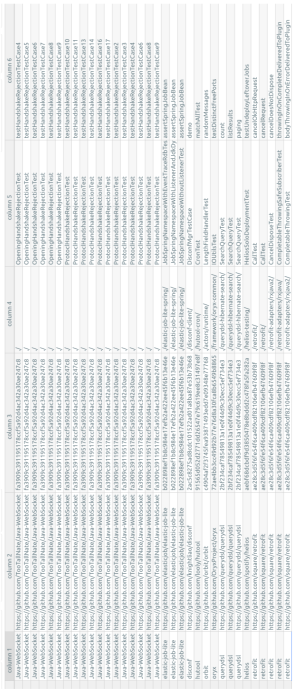
\includegraphics[width=1\textwidth]{3.2}
	\caption{\emph{Esempio di output generato da IDFlakies.sh}}
	\label{fig:outputIDFlakies}
\end{figure}
\subsubsection{FirstStep.sh 2.0}
Per quanto riguarda “FirstStep.sh”, è stato nuovamente sviluppato il
meccanismo per eseguire la build del progetto. In questa nuova versione dello script la build del progetto viene eseguita solo nel momento in cui il repository non è posizionata sul branch di nostro interesse. Per individuare l’attuale branch, viene quindi effettuato il comando di git checkout seguito dallo sha individuato nel file di
input. Se il comando dà esito positivo (ovvero viene segnalato il posizionamento su un nuovo branch), allora viene nuovamente eseguito il comando di mvn install, altrimenti, se dà esito negativo (ovvero, viene segnalato di essere già sul branch desiderato), non viene effettuata la build del progetto. Tale controllo ha permesso
di ottimizzare i tempi di esecuzione in quanto viene effettuata la build del sistema solo in caso di effettiva necessità. Infine, si è deciso di salvare all’interno del file csv di output anche il risultato della build del progetto al fine di rendere disponibile
tale informazione per analisi future.

Di seguito è mostrato il codice per effettuare le operazioni descritte precedentemente.
\lstinputlisting{code/FirstStep.sh}

Il file csv creato da questo script conterrà le seguenti informazioni:
\begin{itemize}
	\item Name Repository;
	\item Link Repository;
	\item Sha della commit;
	\item Build result.
\end{itemize}

La figura \ref{fig:outFirstStep} mostra parte del csv generato in output dal file “outFirstStep.sh”.
\newpage
\begin{figure}[h]
	\centering
	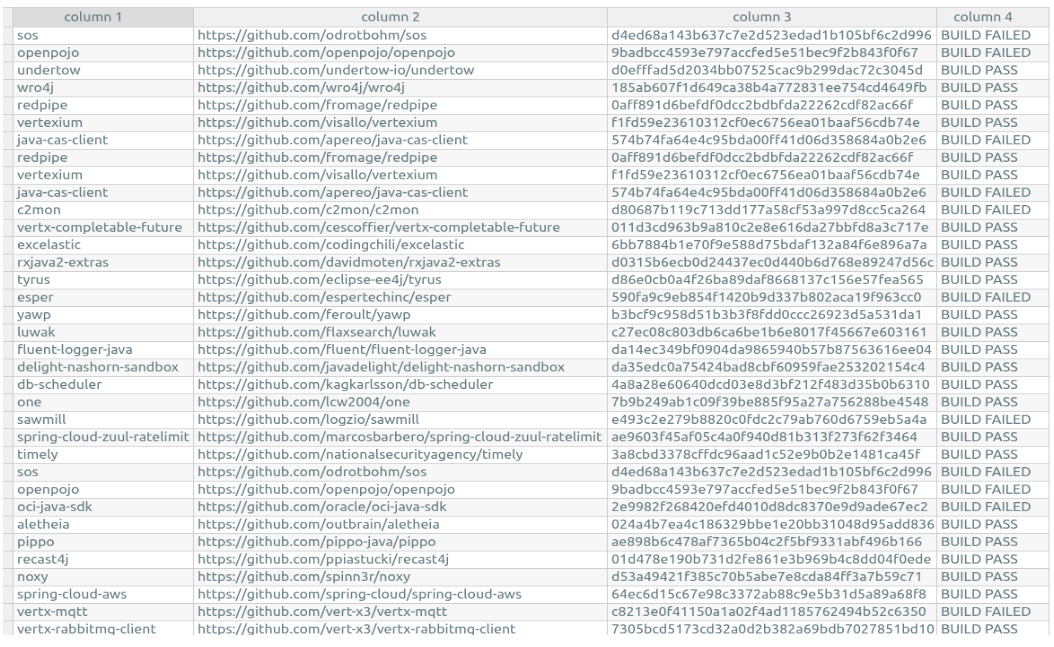
\includegraphics[width=\textwidth]{3.3}
	\caption{\emph{File creato da OutFirstStep.sh}}
	\label{fig:outFirstStep}
\end{figure}
\subsubsection{SecondStep.sh 2.0}
Per ottenere maggiori dettagli dallo script “SecondStep.sh”, si è deciso di generare un file csv intermedio per ogni metodo analizzato. Tale file contiene al suo interno le informazioni sulle N iterazioni eseguite su quel determinato caso di test. Inoltre, si è deciso di salvare su un file di log lo stato della macchina prima e
dopo l’esecuzione del metodo ed il tempo di inizio e quello di fine per ogni esecuzione effettuata, come meglio dettagliato di seguito. Tali metodi hanno permesso di ottenere dei dettagli aggiuntivi che potrebbero servire per una futura analisi. Le informazioni salvate in questo csv intermedio sono:
\begin{itemize}
	\item Name Repository;
	\item Link Repository;
	\item Sha della commit;
	\item Module Name;
	\item Class Name;
	\item Method Name;
	\item Result dell’esecuzione;
	\item Data di inizio esecuzione;
	\item Data di fine esecuzione.
\end{itemize}

La figura \ref{fig:csvIntermedio} mostra un esempio di file csv intermedio. Le informazioni raccolte nel csv intermedio sono state poi riassunte in un csv finale in cui in ogni riga vengono riportate le informazioni sul totale delle iterazioni, sul numero di successi e numero di fallimenti per quel determinato caso di test. In figura \ref{fig:csvFinale} viene riportata un estratto del csv finale generato.
\newpage
\begin{figure}[h]
	\centering
	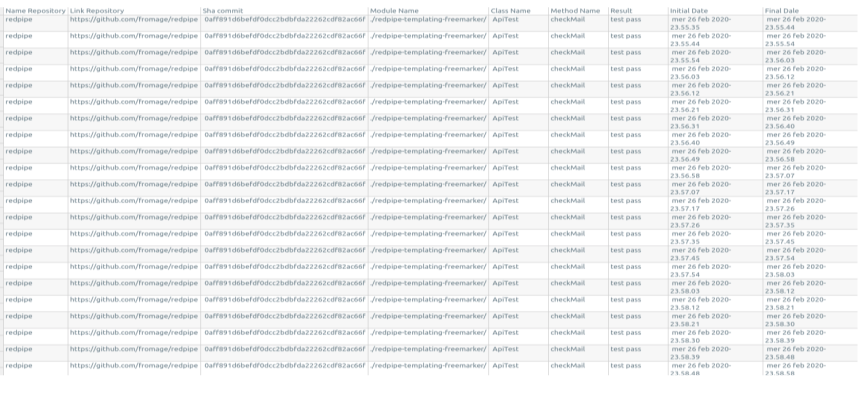
\includegraphics[width=1\textwidth]{3.4}
	\caption{\emph{Esempio del csv intermedio}}
	\label{fig:csvIntermedio}
\end{figure}
\begin{figure}[h]
	\centering
	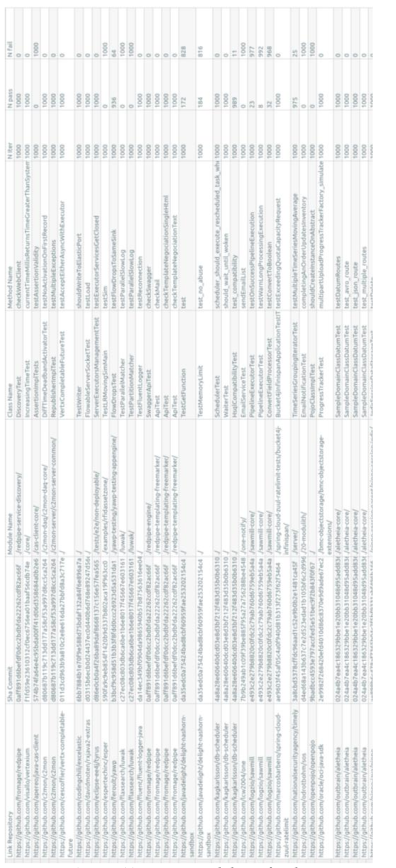
\includegraphics[width=1\textwidth]{3.5}
	\caption{\emph{Esempio del csv finale}}
	\label{fig:csvFinale}
\end{figure}

Di seguito è riportato il codice dello script “secondStep.sh”.
\lstinputlisting{code/SecondStep.sh}

Com’è possibile notare, la funzione \emph{searchFlaky()} si posiziona all’interno del module name indicato nel file csv ed effettua le seguenti operazioni:
\begin{enumerate}
	\item Salva all’interno della variabile timestampInitial il \emph{timestamp} attuale e all’interno della variabile \emph{timestampInitialDate} il timestamp convertito nel
	formato “Date”;
	\item Salva all’interno della variabile stateMachineInitial lo stato attuale della macchina prima dell’esecuzione del test, ottenuto con il comando \emph{vmstat -t};
	\item Esegue il comando \emph{mvn -Dtest=\$concatName test} e salva all’interno di un file di log il risultato;
	\item Riesegue il comando \emph{vmstat -t} per tener traccia dello stato della macchina dopo l’esecuzione del test;
	\item Calcola il nuovo timestamp di fine esecuzione e lo salva nella variabile	\emph{timeStampFinal};
	\item Controlla l’output del comando \emph{mvn -Dtest} per verificare il risultato dell’esecuzione;
	\item Se all’interno dell’output è presente la stringa “\emph{BUILD SUCCESS}” allora verrà incrementato il contatore della variabile \emph{PASSTEST} di una unità, altrimenti verrà incrementato di un’unità il contatore \emph{FAILTEST};
	\item Alla fine di ogni esecuzione vengono salvate le informazioni sul nome e il
	link del repository, lo \emph{sha} della commit, il nome della classe, il nome del metodo, il risultato ottenuto in quella iterazione ed infine il timestamp iniziale e finale entrambi convertiti in formato “Date”.
\end{enumerate}

Una volta terminata la funzione \emph{searchFlaky} viene creato un csv riassuntivo di tutte le varie iterazioni in cui sono riportate le informazioni sul numero totale di test che hanno avuto successo ed il numero totale di test che hanno avuto un fallimento come risultato.
\subsection{Esecuzione degli script su metodi OD}
Sono stati successivamente provati gli script anche sui casi di test etichettati come OD all’interno del csv rilasciato da \textbf{iDFlakies}. Lo scopo di questo test è stato quello di verificare l’effettiva dipendenza dall’ordine di esecuzione dei metodi da loro indicati. Su ogni metodo testato, l’esperimento ha dato esito negativo
(mostrando o tutti “pass” o tutti “fail”). Tale esperimento ha effettivamente comprovato che in quei casi il flaky riscontrato dipendeva dall’ordine in cui veniva eseguito il test, pertanto verranno inseriti all’interno del dataset finale attenendosi
alla classificazione data da \textbf{iDFlakies}.
\subsection{Grafico dei dati ottenuti}
L’ultima operazione effettuata è stata la creazione di grafici per i risultati ottenuti. Per effettuare questa fase sono stati individuati i \emph{flaky test} presenti all’interno del file “finalCSV.csv” e sono stati considerati i corrispettivi file csv
intermedi; si è poi andati a generare i grafici corrispondenti. Per effettuare questa fase è stato creato uno script Python per caricare i dati all’interno di un database e successivamente è stato utilizzato un tool per visualizzarli.
\subsubsection{Creazione dello script}
Lo script Python è stato suddiviso in due moduli. Il primo modulo legge tutto
il contenuto di una directory e genera in output una lista contenente tutti i file in formato csv presenti all’interno. Successivamente tramite un’apposita libreria i dati
sono stati manipolati (es. sostituendo la dicitura: “test pass” con il valore 1 e “test fail” con il valore 0) e poi sono stati passati al modulo denominato “load\_data\_influxDB”. Tale metodo sfruttando le API di InfluxDB carica i dati all’interno del database.
\subsubsection{InfluxDB e Chronograf}
Per l'immagazzinamento dei dati è stato individuato il database “InfluxDB”. Tale database è particolarmente indicato nel momento in cui bisogna rappresentare dati temporali. Nello scegliere il tool da adoperare per graficare i dati
si è optato per “\textbf{Chronograf}” in quanto è un tool sviluppato dalla stessa software
house di InfluxDB.

Di seguito vengono mostrati alcuni dei grafici generati.

Il grafico in figura\ref{fig:AndamentoFlaky} mostra l’andamento del metodo
“\emph{runReconnectBlockingScenario2}” appartenente alla classe “\emph{Issue256Test}” del progetto “\textbf{Java-WebSocket}”.
\begin{figure}[h]
	\centering
	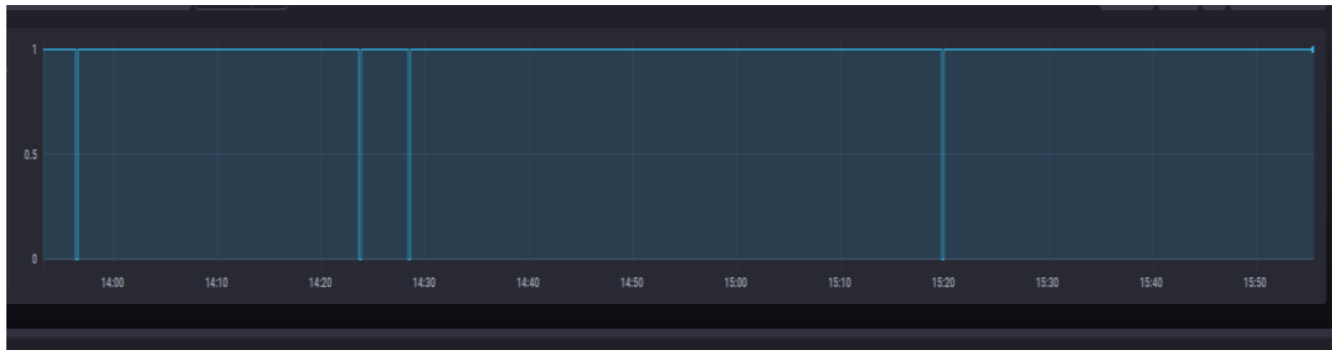
\includegraphics[width=\textwidth]{3.6}
	\caption{\emph{Andamento di uno dei metodi flaky}}
	\label{fig:AndamentoFlaky}
\end{figure}

Com’è possibile osservare dal grafico, tale metodo presenta quattro fallimenti su mille esecuzioni.\newline
Il grafico in figura \ref{fig:fallimentobulk} mostra il fallimento del metodo “\emph{testBulkClusterJoining}” appartenente alla classe “\emph{ZKTest}” del progetto “\textbf{Noxy}”.
\begin{figure}[h]
	\centering
	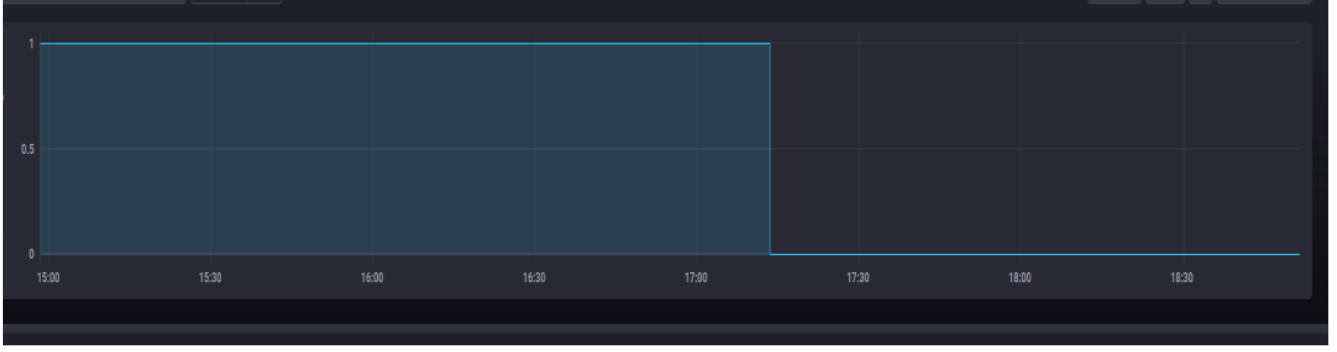
\includegraphics[width=\textwidth]{3.7}
	\caption{\emph{Andamento del metodo testBulkClusterJoining}}
	\label{fig:fallimentobulk}
\end{figure}
\newline
Il metodo preso in esame presentava una serie di successi consecutivi (152) per poi iniziare una serie di fallimenti (848). Il metodo quindi è stato ritestato ma ha dato sempre risultati simili a quello mostrato precedentemente.
L’ultimo metodo che si vuole illustrare è del progetto “timely”. Il metodo in questione è: “\emph{testMultipleTimeSeriesMovingAverage}” appartenente alla classe
“\emph{TimeSeriesGroupingIteratorTest}”. Tale metodo risulta molto interessante poiché mostra un fallimento ogni volta che scatta il 58esimo minuto di un’ora.
La figura 3.8 mostra l’esecuzione del metodo
\begin{figure}[h]
	\centering
	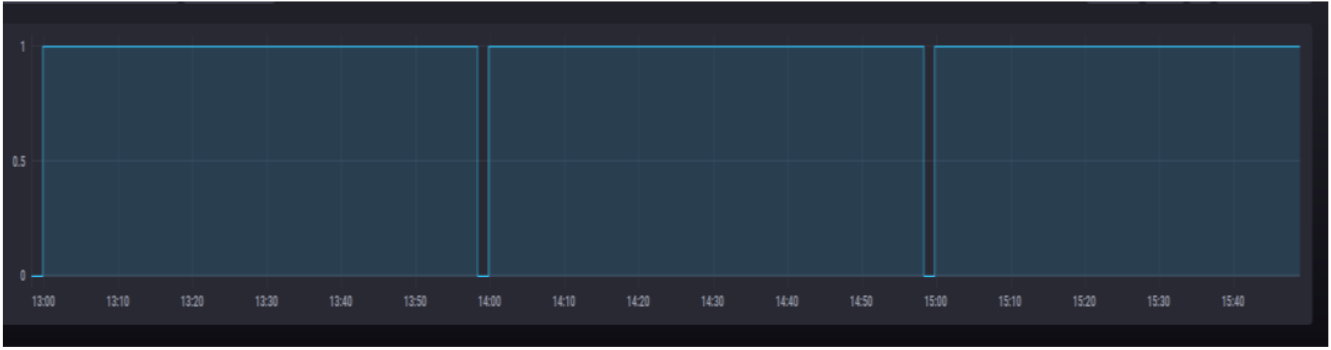
\includegraphics[width=\textwidth]{3.8}
	\caption{\emph{Andamento di testMultipleTimeSeriesMovingAverage}}
	\label{fig:patternFlaky}
\end{figure}
Per ottenere una maggiore sicurezza, si è quindi proceduto ad eseguire altre due volte il metodo sopra elencato.
Le figure \ref{fig:riesecuzione1} e \ref{fig:riesecuzione2} mostrano i risultati delle altre esecuzioni effettuate.
\begin{figure}[h]
	\centering
	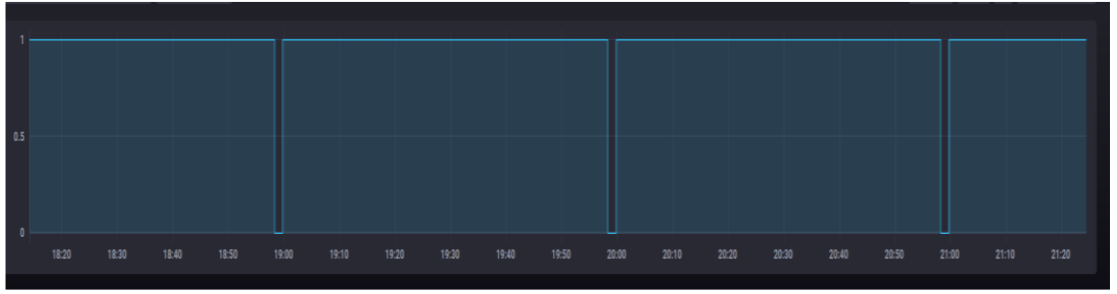
\includegraphics[width=\textwidth]{3.9}
	\caption{\emph{Seconda esecuzione del test in analisi}}
	\label{fig:riesecuzione1}
\end{figure}
\begin{figure}[h]
	\centering
	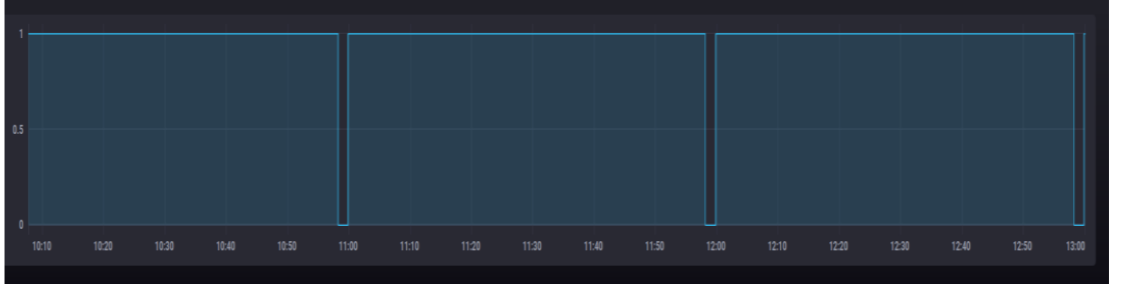
\includegraphics[width=\textwidth]{3.10}
	\caption{\emph{Terza esecuzione del test in analisi}}
	\label{fig:riesecuzione2}
\end{figure}
\newline
Possiamo quindi considerare questo tipo di flaky “deterministico” in quanto presenta un pattern ben preciso.
\subsection{Root cause più frequenti}
Sono state infine analizzate le root cause dei flaky test individuati tramite una
analisi statica del codice. Tale analisi è stata fatta sui repository con comportamenti più “stabili” (ovvero un numero bilanciato sia di “pass” che di “fail”), e sono emersi
i seguenti risultati:
\begin{itemize}
	\item 99\% Errore di Network;
	\item 1\% Multithreading.
\end{itemize}
Tali risultati andrebbero però inquadrati in contesti più ampi e con più dati a disposizione.
\subsection{Limiti della ricerca}
Durante tutta la fase di ricerca sono emersi diversi limiti, alcuni dei quali sono stati trattati precedentemente, altri invece vengono presentati in questa sezione.
\begin{itemize}
\item Lentezza dell’esecuzione della build: In alcuni casi sono state analizzati progetti la cui build ha impiegato oltre due/tre ore per terminare. Tale problematica è sintomo di sistemi di building ancora non adeguatamente efficienti;
\item Lentezza nell’eseguire un singolo caso di test: In alcuni casi sono stati impiegati svariati minuti per eseguire un singolo caso di test; da una indagine effettuata, il sistema di build di Maven riconfigura parte dell’ambiente ad ogni singola esecuzione. Tale riconfigurazione può impiegare anche diversi minuti;
\item Limiti hardware: Gli esperimenti sono stati eseguiti su una macchina Ubuntu 16.04 4GB di RAM 2. Intel Core i3-2100 CPU 3.10GHzx4;
\item Sha non validi: In alcuni casi non c’è stata la possibilità di eseguire l’allineamento sul branch indicato dal dataset in quanto è stato restituito il seguente errore: “reference is not a tree” nel momento in cui è stato eseguito il comando “git checkout”.
\end{itemize}

\chapter*{Conclusioni}
\fancyhf{}
\fancyhead[L]{CONCLUSIONI}
\fancyhead[C]{}
Nella prima parte della tesi è stata effettuato un mapping study sistematico della letteratura. Questa ricerca ha evidenziato una conoscenza ancora in stato embrionale sull’argomento ed in molti casi una carenza di dati. È emerso che nel tempo sono stati rilasciati pochi dataset sulla problematica trattata e prevalentemente di natura open-source. Inoltre, quasi la totalità degli studi si è concentrata su un unico linguaggio di programmazione (\textbf{Java}) e su un unico sistema di building (\textbf{Maven}). Non sempre sono state descritte in maniera accurata le tecniche utilizzate per la costruzione dei dataset (in alcuni casi sono stati riutilizzati dei dataset preesistenti), inoltre le \emph{root cause} sono state individuate in maniera parziale in quanto in alcuni articoli più recenti ne sono comparse di nuove (soprattutto per sistemi operativi mobile) che non erano ancora state individuate.

Si è quindi deciso di contribuire alla costruzione di un nuovo tool per l’identificazione dei \emph{flaky test} indipendenti dall’ordine. Partendo dal dataset già rilasciato dagli sviluppatori di \textbf{iDFlakies}, sono state analizzati centosessantasei casi di test classificati come non dipendenti dall’ordine. Di questi, trentuno hanno mostrato un comportamento “flaky”. Sono state poi analizzate le root cause di questi metodi ed è emerso che nella quasi totalità dei casi (trenta \emph{flaky test}) la \emph{root cause} era legata al network, mentre soltanto per un \emph{flaky test} la \emph{root cause} era legata al multithreading. Il tool ha permesso di ottenere informazioni più dettagliate su particolari metodi “flaky”, come lo stato della macchina prima e dopo l’esecuzione del test e il timestamp di ogni singola iterazione. Inoltre, il tool ha evidenziato anche i limiti degli attuali sistemi di build che in molti casi risultano poco ottimizzati per affrontare adeguatamente lo studio della problematica in esame.

Infine, i risultati sono stati immagazzinati all’interno di una base di dati e sono
stati rappresentati sotto forma di grafici in modo da evidenziare eventuali pattern. Dai risultati è emerso che in alcuni casi è stato riscontrato effettivamente la presenza di un pattern, aprendo la strada all’ipotesi che alcuni flaky test abbiano un comportamento deterministico. I risultati ottenuti dovranno essere ulteriormente approfonditi.
Gli sviluppi futuri del lavoro saranno:
\begin{itemize}
\item “Instrumentation” del codice per poter monitorare ed avere maggiore controllo sui casi di test che sono in esecuzione;
\item Ampliare il tool in modo da poter individuare flaky test dipendenti dall’ordine;
\item Rendere il tool indipendente dal linguaggio di programmazione in cui sono scritti i progetti in analisi.
\end{itemize}
%%%%%%%%%%%%%%%%%%%%%%%%%%%%
\chapter*{Appendice A}
\fancyhead[L]{APPENDICE A}
\fancyhead[C]{}
\fancypagestyle{plain}{%
	\renewcommand{\headrulewidth}{0pt}%
	\fancyhf{}%
}
Di seguito sono riportati i riferimenti bibliografici degli articoli usati per la
revisione sistematica della letteratura.
\newline~\newline
[S1] \textbf{Qingzhou L., Farah H., Lamyaa E., Darko M.} (2014) “An Empirical Analysis of Flaky Tests”. \emph{Proceedings of the 22nd ACM SIGSOFT International Symposium on Foundations of Software Engineering, Hong Kong, China, 2014.}
\newline~\newline
[S2] \textbf{Jonathan B., Gail K., Eric M., Mohan D.} (2015) “Efficient Dependency Detection for Safe Java Test Acceleration”. \emph{Proceedings of the 2015 10th Joint Meeting on Foundations of Software Engineering, Bergamo, Italy, 2015.}
\newline~\newline
[S3] \textbf{Zebao G., Yalan L., Myra B. C., Atif M. M., Zhen W.} (2015) “Making system user interactive tests repeatable: when and what should we control?”. \emph{ICSE‘15: Proceedings of the 37th International Conference on Software Engineering-Volume 1.}
\newline~\newline
[S4] \textbf{Alex G., August S., Farah H., Darko M.}(2015) “Reliable Testing: Detecting State-polluting Tests to Prevent Test Dependency”. \emph{Proceedings of the 2015 International Symposium on Software Testing and Analysis, Baltimore MD, USA, 2015.}
\newline~\newline
[S5] \textbf{Milos G., Lamyaa E., Darko M.} (2015) 
“Practical regression test selection with dynamic file dependencies”. \emph{ISSTA 2015: Proceedings of the 2015
International Symposium on Software Testing and Analysis.}
\newline~\newline
[S6] \textbf{Lam W, Zhang S, Ernst MD}(2015) “When tests collide: Evaluating and coping with the impact of test dependence”.
\newline~\newline
[S7] \textbf{Shi A., Gyori, A., Legunsen O., Marinov D.} (2016) ”Detecting Assumptions on Deterministic Implementations of Non-deterministic Specifications”.\emph{ Proceedings of the 2016 International Conference on Software Testing, Verification and Validation, USA.}
\newline~\newline
[S8] \textbf{Thomas R., Waldemar H., Philipp L., Stefan S.} (2017). “An Empirical Analysis of Build Failures in the Continuous Integration Workflows of Java-based Open-source Software”. \emph{Proceedings of the 14th International Conference on Mining Software Repositories, Buenos Aires, Argentina, 2017.}
\newline~\newline
[S9] \textbf{Candido, J., Melo L., D’Amorim, M.} (2017) “Test suite parallelization in open-source projects: A study on its usage and impact”. \emph{ASE 2017 – Proceedings of the 32nd IEEE/ACM International Conference on Automated Software
Engineering.}
\newline~\newline
[S10] \textbf{Fabio P., Andy Z.} (2015) “Does Refactoring of Test Smells Induce Fixing Flaky Tests?”. \emph{International Conference on Software Maintenance and Evolution, Shanghai, China, 2017.}
\newline~\newline
[S11] \textbf{Labuschagne, A., Inozemtseva, L., Holmes, R.} (2017) “Measuring the cost of regression testing in practice: a study of Java projects using continuous integration”. \emph{Proceedings of the ACM SIGSOFT Symposium on the Foundations of Software Engineering August 2017.}
\newline~\newline
[S12] \textbf{Jonathan B., Owolabi L., Michael H., Lamyaa E., Tifany Y., Darko M.} (2018) “DeFlaker: Automatically Detecting Flaky Tests”. \emph{Proceedings of the 40th International Conference on Software Engineering, Gothenburg, Sweden, 2018.}
\newline~\newline
[S13] \textbf{Swapna T., Chandani S., Na M.} (2018) “An Empirical Study of Flaky Tests in Android”. \emph{International Conference on Software Maintenance and Evolution, Madrid, Spain, 2018.}
\newline~\newline
[S14] \textbf{Md T. R., Peter C. R.} (2018) “The Impact of Failing, Flaky, and High Failure Tests on the Number of Crash Reports Associated with Firefox Builds”. \emph{Proceedings of the 2018 26th ACM Joint Meeting on European Software Engineering Conference and Symposium on the Foundations of Software Engineering, Lake Buena Vista FL, USA, 2018.}
\newline~\newline
[S15] \textbf{Gambi, A., Bell, J., Zeller, A.} (2018) “Practical Test Dependency Detection Proceedings”. \emph{2018 IEEE 11th International Conference on Software Testing, Verification and Validation, ICST 2018.}
\newline~\newline
[S16] \textbf{Eck M., Palomba F., Castelluccio M., Bacchelli A.} (2019)
“Understanding Flaky Tests: The Developer’s Perspective”. \emph{Proceedings of the 2019 27th ACM Joint Meeting on European Software Engineering Conference and Symposium on the Foundations of Software Engineering, Tallinn, Estonia, 2019.}
\newline~\newline
[S17] \textbf{Wing L., Patrice G., Suman N., Anirudh S., Suresh T.} (2019) “Root Causing Flaky Tests in Large-scale Industrial Setting”. \emph{Proceedings of the 28th ACM SIGSOFT International Symposium on Software Testing and Analysis, Beijing, China, 2019.}
\newline~\newline
[S18] \textbf{Armin N., Peter C. R.,Weiyi S.} (2019) “Bisecting commits and modeling commit risk during testing”. \emph{ESEC/FSE 2019: Proceedings of the 2019 27th ACM Joint Meeting on European Software Engineering Conference and Symposium on the Foundations of Software Engineering.}
\newline~\newline
[S19] \textbf{Kai Presler-M., Eric H., Sarah H., Kathryn S.} (2019) “Wait, Wait. No, Tell Me. Analysing Selenium Configuration Effects on Test Flakiness”. \emph{14th International Workshop on Automation of Software Test, Montreal, QC, Canada, 2019.}
\newline~\newline
[S20] \textbf{August S., Wing L., Reed O., Tao X., Darko M.} (2019) ”iFixFlakies: A Framework for Automatically Fixing Order-dependent Flaky Tests” \emph{In Proceedings of the 2019 27th ACM Joint Meeting on European Software Engineering Conference and Symposium on the Foundations of Software Engineering, Tallinn, Estonia, 2019.}
\newline~\newline
[S21] \textbf{Biagiola M., Stocco A., Mesbah A., Ricca F., Tonella P.} (2019) “Web test dependency detection”. \emph{ESEC/FSE 2019: Proceedings of the 2019 27th ACM Joint Meeting on European Software Engineering Conference and Symposium on the Foundations of Software Engineering.}
\newline~\newline
[S22] \textbf{August S., Jonathan B., Darko M.} (2017) “Mitigating the Effects of Flaky Tests on Mutation Testing”. \emph{Proceedings of the 28th ACM SIGSOFT International Symposium on Software Testing and Analysis, Beijing, China, 2017.}
\newline~\newline
[S23] \textbf{Andreas S., Marvin K., Gordon F.} (2019) “Testing Scratch Programs Automatically”. \emph{Proceedings of the 2019 27th ACM Joint Meeting on European Software Engineering Conference and Symposium on the Foundations of Software Engineering, Tallinn, Estonia, 2019.}
\newline~\newline
[S24] \textbf{Pontes F., Gheyi R., Souto S., Garcia A., Ribeiro M.} (2019) “Java reflection API: revealing the dark side of the mirror”. \emph{ESEC/FSE 2019: Proceedings of the 2019 27th ACM Joint Meeting on European Software Engineering Conference and Symposium on the Foundations of Software Engineering.}
\newline~\newline
[S25] \textbf{Böhme M.} (2019) “Assurance in software testing: a roadmap”. \emph{ICSE- NIER ‘19: Proceedings of the 41st International Conference on Software Engineering: New Ideas and Emerging Results.}
\newline~\newline
[S26] \textbf{Schwahn O., Coppik N., Winter S., Suri N.} (2019) “Assessing the state and improving the art of parallel testing for C”. \emph{ISSTA 2019: Proceedings of the 28th ACM SIGSOFT International Symposium on Software Testing and Analysis.}
\newline~\newline
[S27] \textbf{Zhiyu F.} (2019) “A Systematic Evaluation of Problematic Tests Generated by EvoSuite”. \emph{41st International Conference on Software Engineering: Companion Proceedings, Montreal, QC, Canada, 2019.}
\newline~\newline
[S28] \textbf{Wing L., Reed O., August S., Darko M., Tao X.} (2019) “iDFlakies: A Framework for Detecting and Partially Classifying Flaky Tests”. \emph{12th IEEE Conference on Software Testing, Validation and Verification, Xi’an, China, 2019.}
\newline~\newline
[S29] \textbf{Morán, J., Augusto, C., Bertolino, A., De La Riva, C., Tuya, J.}
(2019) “Debugging flaky tests on web applications” \emph{WEBIST 2019-Proceedings of the 15th International Conference on Web Information Systems and Technologies.}
\newline~\newline
[S30] \textbf{Palomba F., Zaidman A.} (2019)” The Smell of Fear: On the Relation Between Test Smells and Flaky Tests”. \emph{Empirical Software Engineering, Salerno, Italy, 2019.}
\fancypagestyle{plain}{%
	\renewcommand{\headrulewidth}{0pt}%
	\fancyhf{}%
}
\bibliographystyle{unsrt}
\bibliography{Reference} % bibliografia
\chapter*{Sitografia}
\fancyhead[L]{SITOGRAFIA}
\fancyhead[C]{}
\fancypagestyle{plain}{%
	\renewcommand{\headrulewidth}{0pt}%
	\fancyhf{}%
}
\textsuperscript{[1]} \textbf{Android FlakyTest annotation}\\
\url{https://developer.android.com/reference/android/test/FlakyTest.html}\\
(Ultimo accesso: Gennaio 2020)
\newline~\newline
\textsuperscript{[2]} \textbf{No more flaky tests on the Go team}\\
\url{https://www.thoughtworks.com/insights/blog/no-more-flaky-tests-go-team}\\
(Ultimo accesso: Febbraio 2020)
\newline~\newline
\textsuperscript{[3]} \textbf{Flaky Tests at Google and How We Mitigate Them}\\
\url{https://testing.googleblog.com/2016/05/flaky-tests-at-google-and-how-we.html}\\
(Ultimo accesso: Gennaio 2020)
\newline~\newline
\textsuperscript{[4]} \textbf{Rerun Failing Tests}\\
\url{https://maven.apache.org/surefire/maven-surefire-plugin/examples/rerun-failing-tests.html}\\
(Ultimo accesso: Febbraio 2020)
\newline~\newline
\textsuperscript{[5]} \textbf{Flaky Test Handler v1.04}\\
\url{https://plugins.jenkins.io/flaky-test-handler/}\\
(Ultimo accesso: Gennaio 2020)
\newline~\newline
\textsuperscript{[6]} \textbf{TotT: Avoiding Flakey Tests}\\
\url{https://testing.googleblog.com/2008/04/tott-avoiding-flakey-tests.html}\\
(Ultimo accesso: Febbraio 2020)
\\

\chapter*{Ringraziamenti}
\fancyhead[L]{}
\fancyhead[C]{}

Giunto oramai al termine del mio percorso di studio è doveroso soffermarsi un attimo su tutte le persone che mi sono state vicine in questo periodo.
\newline~\newline
In primis vorrei ringraziare la professoressa Ferrucci che è stata per me oltre che una docente una guida durante tutto il mio percorso accademico. Senza i suoi consigli e senza i suoi insegnamenti tutto ciò non sarebbe stato possibile.
\newline~\newline
Desidero inoltre ringraziare i Dottori Pasquale Salza e Valerio Terragni che hanno saputo ascoltare i miei dubbi e soprattutto mi hanno aiutato con brillanti consigli e sincere opinioni.
\newline~\newline
Ringrazio la mia ragazza Raffaella che ha saputo ancora una volta
supportarmi/sopportami durante tutto il mio percorso accademico. Grazie per tutti i consigli e per tutto ciò che hai fatto in questi anni per me.
\newline~\newline
Ringrazio Valeria che ha affrontato con me praticamente ogni esame di questa magistrale e con cui ho condiviso non solo l’università ma questi ultimi due anni. La tua sincera amicizia e le ore interminabili di studio mi hanno permesso di arrivare a realizzare tutto ciò.
\newline~\newline
Inoltre, desidero ringraziare tutti i miei, amici Diego e Francesco il primis per aver condiviso con me interminabili momenti di divertimento misto a studio matto e disperato. 
\newline~\newline
Un ringraziamento particolare va a Salvatore che ancora una volta mi ha saputo aiutare e con cui ho trascorso momenti di puro divertimento al di fuori dell’università.
\newline~\newline
Desidero ringraziare Anna che mi ha aiutato in quest’ultimo periodo consigliandomi e aiutandomi in ogni momento.
\newline~\newline
Infine, i miei amici di una vita Cosimo, Giuseppe, Giovanni, Raimondo (con cui ho condiviso ogni mio WTF) e Vincenzo che ancora una volta si sono dimostrati dei
veri amici.
\newline~\newline
Ringrazio la mia famiglia e mio fratello Benito che mi hanno sempre
supportato in ogni mia decisione senza mai farmi pesare nessuno dei sacrifici che hanno dovuto sostenere per me in tutti questi anni.
\newline~\newline
Infine, ringrazio la mia seconda famiglia Salvatore e Michela che mi hanno sempre incoraggiato ad andare oltre ciò che avevo per puntare sempre ad obiettivi più ambiziosi e le gemelle Katia e Alessia che mi hanno accolto come uno di famiglia.

\begin{flushright}
Grazie a tutti voi...
\end{flushright}
\end{document}
